\section{Deep Learning}
\label{sec:bg.dl}

When attempting to tackle a task computationally, it is common to explicitly define an algorithm that solves the task in a structured way with manually set parameters. In practice, this approach is often unfeasible for complex tasks with high-dimensional data, such as image generation or speech recognition. A different approach is \emph{machine learning}, i.e., to assemble a dataset of correct inputs and outputs and defining an algorithm which exploits statistical correlations in the dataset to fit a model that generalizes to data outside of this dataset. \emph{Deep learning} is a subset of machine learning that has gained traction in recent years due to practical successes \citep{DBLP:conf/cvpr/CiresanMS12,DBLP:conf/nips/KrizhevskySH12, DBLP:journals/nature/SilverHMGSDSAPL16,DBLP:conf/naacl/DevlinCLT19,DBLP:conf/nips/BrownMRSKDNSSAA20,DBLP:conf/cvpr/RombachBLEO22,DBLP:journals/corr/abs-2203-02155}.

The basis of deep learning are \emph{neural networks} \citep{Rosenblatt58theperceptron}, which are explained in \Cref{subsec:bg.nn}. Different ways of formulating objectives for and measuring neural networks are explored in \Cref{subsec:bg.losses}. \Cref{subsec:bg.cnn} describes \glspl{cnn} \citep{DBLP:journals/pr/FukushimaM82,10.1162/neco.1989.1.4.541}, which are a type of neural networks suited for spatial data such as raster images. The equivalent for sequential data, \glspl{rnn} \citep{Rumelhart1986}, are detailed in \Cref{subsec:bg.rnn}. The Transformer architecture \citep{DBLP:conf/nips/VaswaniSPUJGKP17,schmidhuber1992learning}, a recently developed model architecture attempting to combine the advantages of \glspl{cnn} and \glspl{rnn} is introduced in \Cref{subsec:bg.tf}. \Cref{subsec:bg.vae} describes a flexible framework for generative models called encoder-decoder framework \citep{DBLP:conf/nips/SutskeverVL14,FITPT283}.


\subsection{Neural Networks}
\label{subsec:bg.nn}

\begin{figure}[h]
\centering
\begin{tikzpicture}
    \node[circle, draw, fill=lightgray] (x0) at (0,0.5) {$x_0$};
    \node[circle, draw, fill=lightgray] (x1) at (0,1.5) {$x_1$};
    \node[circle, draw, fill=lightgray] (x2) at (0,2.5) {$x_2$};
    \node[circle, draw] (h0) at (4,0) {$h_0$};
    \node[circle, draw] (h1) at (4,1) {$h_1$};
    \node[circle, draw] (h2) at (4,2) {$h_2$};
    \node[circle, draw] (h3) at (4,3) {$h_3$};
    \node[circle, draw, fill=gray] (o0) at (8,1) {$o_0$};
    \node[circle, draw, fill=gray] (o1) at (8,2) {$o_1$};
    \draw [->] (x0) to (h0);
    \draw [->] (x0) to (h1);
    \draw [->] (x0) to (h2);
    \draw [->] (x0) to (h3);
    \draw [->] (x1) to (h0);
    \draw [->] (x1) to (h1);
    \draw [->] (x1) to (h2);
    \draw [->] (x1) to (h3);
    \draw [->] (x2) to (h0);
    \draw [->] (x2) to (h1);
    \draw [->] (x2) to (h2);
    \draw [->] (x2) to (h3);
    \draw [->] (h0) to (o0);
    \draw [->] (h0) to (o1);
    \draw [->] (h1) to (o0);
    \draw [->] (h1) to (o1);
    \draw [->] (h2) to (o0);
    \draw [->] (h2) to (o1);
    \draw [->] (h3) to (o0);
    \draw [->] (h3) to (o1);
    \node[draw, above=of x2, fill=lightgray] {input};
    \node[draw, above=of h3] {hidden};
    \node[draw, above=of o1, fill=gray] {output};
    \node at (0,-1) {$\textbf{x}$};
    \node at (2,-1) {$\boldsymbol{\theta}_{in}$};
    \node at (4,-1) {$\textbf{x}^T\boldsymbol{\theta}_{in}$};
    \node at (6,-1) {$\boldsymbol{\theta}_{h}$};
    \node at (8,-1) {$f_a(\textbf{x}^T\boldsymbol{\theta}_{in})\boldsymbol{\theta}_{h}$};
\end{tikzpicture}
    \caption{Architecture of a \gls{mlp}. Circles of same color represent the variables within a layer, while the connections between circles indicates weights. The mathematical representation is given below.}
    \label{fig:mlp}
\end{figure}

Consider a set of input data $\textbf{x}\in\mathbb{R}^m$ and a set of outputs $\textbf{y}\in\mathbb{R}^l$ of unspecified dimensions, which are related by the ground truth function $F(\textbf{x})=\textbf{y}, F: \mathbb{R}^m \rightarrow \mathbb{R}^l$. In the context of \emph{machine learning}, $\textbf{x}$ can be referred to as \emph{predictors} and $\textbf{y}$ as the \emph{response} or \emph{label}. For example, in the case of binary image classification the predictor could be a sequence of the color values of all pixels in an image, while the response could be a dichotomous variable indicating whether the image is part of the positive class. The objective of a machine learning algorithm is to fit a model $f$ that approximates $F$ using freely changeable (or, \emph{learnable}) parameters $\boldsymbol{\theta}$, i.e., $f(\textbf{x};\boldsymbol{\theta})\approx F(\textbf{x})$.

Neural networks \citep{Rosenblatt58theperceptron} can be viewed as special, nonlinear case of the approximation $f$. Specifically, a neural network consists of three types of layers:
\begin{itemize}
	\item One input layer $\textbf{x}$
    \item $n$ hidden layers and
	\item one output layer \textbf{o}
\end{itemize}

Intuitively, each hidden layer learns to detect important features of the preceding layer. These features are then used in the last layer - the output layer - to compute the relevant, task dependent outcome.

The  standard feedforward neural network, the \gls{mlp}, is depicted in \Cref{fig:mlp}. Note that \Cref{fig:mlp} depicts a neural network with only one hidden layer. Theoretically, this 1-layered \gls{mlp} is able to approximate any function \citep{DBLP:journals/nn/HornikSW89,DBLP:journals/mcss/Cybenko89}. However, in practice, it has been shown that neural networks that consist of many hidden layers perform better on complex functions \citep{DBLP:journals/tc/Amari67,DBLP:conf/icml/SafranS17,DBLP:journals/nn/PetersenV18}. The amount of hidden layers is also referred to as the \emph{depth} of the neural network, leading to the term \emph{deep learning}  \citep{DBLP:conf/aaai/Dechter86,DBLP:journals/tnn/ChenKKH01a}.

In the \gls{mlp} architecture, each hidden layer consists of a predetermined size $k$ of nodes. Every node is connected to all nodes of the preceding layer (hence also called \emph{fully connected}). Each of these connections is assigned a learnable weight $\theta$. Thus, the value of each node is the weighted sum of all nodes of the preceding layer. Therefore, each layer in a neural network can be described as inner product $\textbf{h}=\textbf{x}^T \boldsymbol{\theta}$, where $\textbf{x}$ is the vector of nodes of the preceding layer and $\boldsymbol{\theta}\in \mathbb{R}^{k\times|\textbf{x}|}$ is a matrix, where $\boldsymbol{\theta}_i \forall i \in [0,k]$ is a vector of weights for one node. For brevity, the bias term is omitted. Intuitively, each node is a specific \emph{representation} of the preceding layer which assigns a certain importance (i.e., weight) to every node of the preceding layer.

After the node values of the hidden layer are computed, an \emph{activation function} $\phi(x)$ is applied on them. Early \glspl{mlp} were inspired by biological neural networks and used the sigmoid activation function defined in \Cref{eq:sigmoid}. This function is depicted in \Cref{fig:activationfunctions.sigmoid}. A similar activation function is the tanh activation function defined in \Cref{eq:tanh} and depicted in \Cref{fig:activationfunctions.tanh}. Contemporary neural networks mainly use the \gls{relu} activation function \citep{Nair:2010:RLU:3104322.3104425} defined in \Cref{eq:relu} and depicted in \Cref{fig:activationfunctions.relu}. 

\begin{equation}
\label{eq:sigmoid}
\sigma(x)=1/(1+\exp(-x))
\end{equation}

\begin{equation}
\label{eq:tanh}
\tanh(x)={\frac {\sinh(x)}{\cosh(x)}}={\frac {e^{x}-e^{-x}}{e^{x}+e^{-x}}}
\end{equation}

\begin{equation}
\label{eq:relu}
\text{relu}(x)=\max(0,x)
\end{equation}

\begin{figure}
\centering
    \begin{subfigure}[b]{0.3\textwidth}
        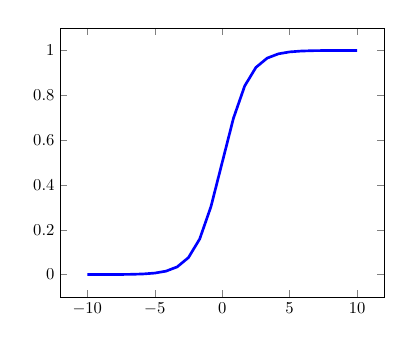
\begin{tikzpicture}[scale=0.6]
            \begin{axis}
                \addplot[domain=-10:10, blue, ultra thick] {1/(1+exp(-x))};
            \end{axis}
        \end{tikzpicture}
        \caption{Sigmoid function.}
        \label{fig:activationfunctions.sigmoid}
    \end{subfigure}
    \hfill
    \begin{subfigure}[b]{0.3\textwidth}
        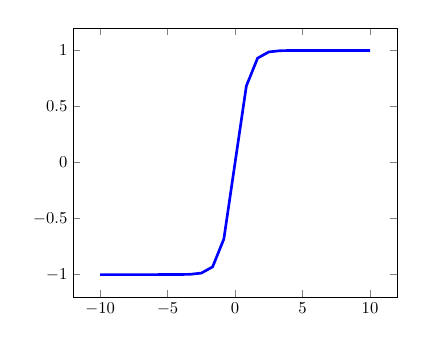
\begin{tikzpicture}[scale=0.6]
            \begin{axis}
                \addplot[domain=-10:10, blue, ultra thick] {(e^(x)-e^(-x))/(e^(x)+e^(-x))};
            \end{axis}
        \end{tikzpicture}
        \caption{Tanh activation function.}
        \label{fig:activationfunctions.tanh}
    \end{subfigure}
    \hfill
    \begin{subfigure}[b]{0.3\textwidth}
        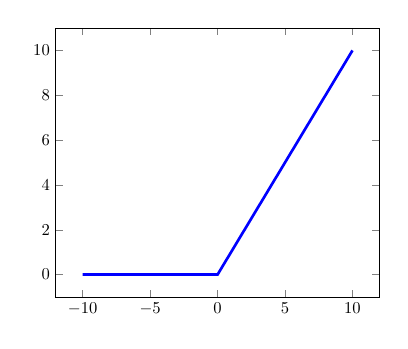
\begin{tikzpicture}[scale=0.6]
            \begin{axis}
                \addplot[domain=-10:10, blue, ultra thick] {max(0,x)};
            \end{axis}
        \end{tikzpicture}
        \caption{\gls{relu} activation function.}
        \label{fig:activationfunctions.relu}
    \end{subfigure}
    \caption{Graphs depicting activation functions.}
    \label{fig:activationfunctions}
\end{figure}

The output of each hidden layer is thus $\phi(\textbf{h})=\phi(\textbf{x}^T \boldsymbol{\theta})$. Notice that $\phi$ serves as nonlinearity. If $\phi$ was not used, the output of an $n$-layered neural network could be computed using $\textbf{o} = \textbf{x}^T \prod_{i=0}^{n}\boldsymbol{\theta}_i=\textbf{x}^T \boldsymbol{\theta}$. This is equivalent to the multiple linear regression model $\textbf{y}=\textbf{x}^T \boldsymbol{\beta} + \boldsymbol{\epsilon}$.

With the activation function $\phi(x)$, a two-layered \gls{mlp} is defined by \Cref{eq:mlp.2l}.

\begin{equation}
\label{eq:mlp.2l}
	\textbf{o} = \phi(\phi(\textbf{x}^T \boldsymbol{\theta}_{\text{in}})\boldsymbol{\theta}_{\text{h}})
\end{equation}

In \Cref{eq:mlp.2l} $\boldsymbol{\theta}_{\text{in}}$ are the connection weights between the input and the hidden layer and $\boldsymbol{\theta}_{\text{h}}$ are the connection weights between the hidden and the output layer.

\subsubsection{Optimization}
\label{subsec:bg.nn.optim}
In order to approximate the ground truth function $F(\textbf{x})$ using the model $f(\textbf{x};\boldsymbol{\theta})$, the optimal parameters $\boldsymbol{\theta}^\star$ have to be found. In machine learning parlance, this is referred to as \emph{fitting}, or \emph{training} the model. In the case of neural networks, this means finding the optimal parameters $\boldsymbol{\theta}^\star_i$ for each hidden layer, such that $f(\textbf{x}; \boldsymbol{\theta}^\star) \approx F(\textbf{x})$. Historically, fitting neural networks often failed to converge to optimal parameters \citep{perceptrons}. However, this changed with the introduction of the backpropagation algorithm (also referred to as reverse-mode differentiation) \citep{Dreyfus_1962, linnainmaa}, which made it possible to efficiently train neural networks.

The first step in optimization is \emph{weight initialization}, i.e., to initialize the learnable parameters $\boldsymbol{\theta}_i$ with random numbers. Next, the output of the neural network is computed as $\textbf{o}=f(\textbf{x}; \boldsymbol{\theta})$. In order to evaluate the output of the network, a \emph{loss function} is defined as $L(\textbf{o},\textbf{y})$. $L$ calculates the error between $\textbf{o}$ and the ground truth $\textbf{y}$. It is important to choose a proper loss function fitting the specific task. A simple loss function sometimes used in image generation is the mean squared error, or $L^2$ distance, defined by \Cref{eq:mse}.

\begin{equation}
    \label{eq:mse}
    L^2(\textbf{o}, \textbf{y}) = \frac{\sum_{i=1}^{|\textbf{o}|} (o_i - y_i)^2}{|\mathbf{o}|}
\end{equation}

Using the \gls{sgd} algorithm, the loss function $L$ can be used to \emph{guide} the training process towards optimal parameters. This is done by computing the gradients $\partial L / \partial \boldsymbol{\theta}_i$ for each weight parameter using backpropagation. These gradients indicate how the loss $L$ changes when $\boldsymbol{\theta}_i$ is increased by an infinitesimal amount. As the loss function needs to be \emph{minimized}, the parameters are updated using the \gls{sgd} update step defined by \Cref{eq:sgd}.

\begin{equation}
\label{eq:sgd}
        \boldsymbol{\theta}_i = \boldsymbol{\theta}_i - \eta \frac {\partial L} {\partial \boldsymbol{\theta}_i}
\end{equation}

$\eta$ in \Cref{eq:sgd} is a hyperparameter called \emph{learning rate} or \emph{step size}. It controls the magnitude of the weight parameter updates and is often a small positive number, as higher numbers quickly lead to exploding or vanishing gradients \citep{hochreiterdipl}.

The \gls{sgd} update step, i.e., computing the outputs and changing the parameters is repeated until a set of parameters that results in a sufficiently small loss is found. In recent times, several enhancements to the \gls{sgd} algorithm were proposed. Most of them are \emph{adaptive} optimization algorithms, i.e., they adapt the learning rate $\eta$ according to the previous gradients or parameter updates. Chief among them are Adam \citep{DBLP:journals/corr/KingmaB14}, AdamW \citep{DBLP:conf/iclr/LoshchilovH19} and RMSprop \citep{rmsprop}. While it is still unproven that these optimization algorithms are strictly better than \gls{sgd} \citep{DBLP:conf/icml/HardtRS16, NIPS2017_7003}, they do perform better on some tasks and model architectures \citep{DBLP:conf/emnlp/LiuLGCH20,DBLP:conf/nips/Anil0KS19}.

For the optimization process to work, it is crucial that the gradients required for the update step $\partial L / \partial \boldsymbol{\theta}_i$ can actually be computed. This means that the loss function $L(\textbf{o},\mathbf{y})$ needs to be \emph{differentiable}, i.e., there must be a derivative at all points in its domain. Since $\textbf{o}=f(\textbf{x}; \boldsymbol{\theta})$ and since the gradients are computed directly with respect to individual $\boldsymbol{\theta}_i\in\boldsymbol{\theta}$, it follows that the model $f$ itself also needs to be differentiable. As an aside, the \gls{relu} activation function defined in \Cref{eq:relu} is actually not differentiable at $x=0$. In order to enable it to be used in the model anyways, the derivative at $x=0$ is arbitrarily set to $0$ ($\text{relu}'(0)=0$).

\subsubsection{Regularization}
\label{subsec:bg.nn.reg}

A common occurrence while training neural networks is \emph{overfitting}, i.e., finding parameters $\boldsymbol{\theta}$ that closely fit the data used to train the network, but do not generalize to unseen data. In order to prevent this, several regularization schemes are employed.

\paragraph{Model and Dataset Size}
In general, the larger a model is (i.e., the more freely changeable parameters $\theta$ it contains) in relation to the dataset size, the easier it is to overfit. Therefore, an important design decision to reduce overfitting is to either reduce the model parameters to the smallest capacity required to converge or to increase the dataset size.

\paragraph{Weight initialization}
Weight initialization is an important decision for the training process, as wrongly initialized neural networks do not converge to a sufficient result \citep{pmlr-v9-glorot10a,Sutskever:2013:IIM:3042817.3043064}. Therefore, one often draws the initial weights of each hidden layer from a Gaussian distribution $\boldsymbol{\theta}_i \sim \mathcal{N}(0,1)$ and scales the variance with a constant. One commonly used method is Xavier initialization \citep{pmlr-v9-glorot10a}, which scales the random numbers by $2/(n_{\text{pre}} + n_{\text{next}})$, where $n_{\text{pre}}$ is the number of nodes of the preceding layer and $n_{\text{next}}$ is the number of nodes in the succeeding layer. Another initialization scheme specifically designed for \gls{relu} neural networks is He initialization \citep{He:2015:DDR:2919332.2919814} with a scale factor of $\sqrt{2/n}$, where $n$ is the number of nodes of each hidden layer.

\paragraph{Batch normalization}
\label{subsec:bg.nn.batchnorm}
Neural networks are normally fitted by processing subsets of the training dataset - \emph{batches} - in parallel. This is primarily done to utilize the nature of \glspl{gpu} in order to speed up the training process. However, it is also possible to use batch statistics to normalize individual observations with respect to the batch. This \emph{batch normalization} \citep{pmlr-v37-ioffe15} ensures that batches are normally distributed, which might improve the stability of the training process. The authors claim that internal covariate shift - i.e., differing distributions of intermediate layer outputs - are detrimental to convergence. However, there exist alternative explanations for how batch normalization actually brings about its regularizing effects in practise \citep{NEURIPS2018_905056c1, DBLP:conf/iclr/YangPRSS19, DBLP:conf/aistats/KohlerDLHZN19}.

More specifically, given a batch $\textbf{x}_B \subset \textbf{x}$, each observation $x_i \in \textbf{x}_B$ is centered using the batch mean $\mu_{B}={\frac {1}{m}}\sum _{i=1}^{m}x_i$ and scaled by the batch variance $\sigma _{B}^{2}={\frac {1}{m}}\sum _{i=1}^{m}(x_i-\mu_{B})^{2}$ as given by \Cref{eq:batchnorm}. In this equation, $k$ denotes the dimension, since batch normalization is applied per-dimension.

\begin{equation}
    \label{eq:batchnorm}
    \hat {x}_{i}^{(k)}={\frac {x_{i}^{(k)}-\mu _{B}^{(k)}}{\sqrt {\left(\sigma _{B}^{(k)}\right)^{2}+\epsilon }}}
\end{equation}

\paragraph{Dropout}
Another way to regularize neural networks and reduce overfitting is to randomly set individual nodes in hidden layers to 0. This technique is called \emph{dropout} \citep{DBLP:journals/corr/abs-1207-0580} and makes the model more robust with respect to individual nodes and their connection weights, since it can not rely on the node value being present.

Dropout is mainly applied while fitting the model. Consider the hidden layer $\textbf{h}=\textbf{h}_{-1}\boldsymbol{\theta}$. After computing the hidden layer nodes $\textbf{h}$ using the preceding layer $\textbf{h}_{-1}$  and the connection weights $\boldsymbol{\theta}$, each node $h \in \textbf{h}$ is independently set to 0 with probability $p$ (it is common to set $p=0.5$). Since this is independently done for every step of the optimization process, different nodes will be "dropped" at each step. Hence, in order to maximize the optimization objective, the connection weights have to be fitted in a way that is robust to a share $p$ of the nodes randomly being dropped (and thereby a share $p$ of the weights not contributing to the output).

\subsection{Metrics and Losses}
\label{subsec:bg.losses}
Recall that a machine learning model $f(\mathbf{x};\boldsymbol{\theta})=\mathbf{o}$ approximates a ground truth function $F(\textbf{x})=\textbf{y}$ by being fitted to an input dataset $(\mathbf{x},\mathbf{y})$ in order to produce outputs $\mathbf{o}$ that fit the ground truth output (or, response) $\mathbf{y}$. It follows, that there is a need for a single numerical value to measure this fit. There are two ways this value is calculated and used in relation to a machine learning model: firstly, to evaluate the model after it has been trained using \emph{metrics} (often against other models or baselines) and secondly, in order to guide the training process using \emph{loss functions}. This section introduces these related concepts.

\subsubsection{Classification}
\label{subsubsec:classification}
Since metrics and losses formulate the objective, they depend on the task of the model. Machine learning tasks can be roughly divided into two categories by the nature of the response $\mathbf{y}$. While in regression tasks, $\mathbf{y}$ is continuous, in classification tasks $\mathbf{y}$ is discrete.

Regression does not impose strict assumptions on $\mathbf{y}$ is therefore the standard case introduced in \Cref{subsec:bg.nn}. An important image-related task that roughly falls into this category is image generation, i.e., to generate output images $\mathbf{o}$ that look similar to the ground truth $\mathbf{y}$.

On the other hand, classification has more strict assumptions on $\mathbf{y}$. The task is to assign to an input $\mathbf{x}$ a predefined class out of $S$ classes. Since machine learning models operate on vectors, the class in the ground truth is represented as a vector $\mathbf{y}\in\mathbb{R}^S$, where each element $y_i\in\mathbf{y}$ is an indicator of the class $i\in[1,S]$. If the input is assigned class $s$, $y_s=1$ and $y_j=0\forall j\in[1,S]$ except $j=s$. Appropriately, the output of the model $\mathbf{o}$ has the same structure as the ground truth $\mathbf{y}$, except it usually consists of continuous class \emph{probabilities} instead of categorical class indicators, i.e., whereas $y_i\in\{0,1\}$, $o_i\in[0,1]$. In the case of binary classification, i.e., if $S=2$, the two class probabilities are exactly the inversion of each other and can be reduced to a single probability, i.e., in this case the class is represented by a single number.

There are image-related tasks that can be framed as classification tasks. Consider the case of image segmentation, which has the objective of partitioning an image into multiple segments, where each segment belongs to one of multiple classes. All regions of a class share certain task-dependent characteristics. \Cref{fig:segmentation} shows an example of an image segmentation task. This example depicts a binary image segmentation task where the image has to be segmented into two classes: segments that correspond to circles and the rest.

\begin{figure}
    \centering
    \includegraphics[width=\textwidth]{graphics/segmentation.pdf}
    \caption{An example of image segmentation, where the circles in the image have to be segmented.}
    \label{fig:segmentation}
\end{figure}

In other words, the output of a segmentation model assigns a class to each pixel of the input image. Given an input image $\mathbf{x}\in\mathbb{R}^{W\times H\times C}$ of width $W$, height $H$ and $C$ color values per pixel, the output is $\mathbf{o}\in\mathbb{R}^{W\times H\times S}$, where $S$ is the number of classes. In detail, each pixel $\mathbf{x}_{i,j}\in\mathbf{x}$ at location $(i,j)$ in the input image $\mathbf{x}$ is assigned a vector $\mathbf{o}_{i,j}\in\mathbf{o}$ of length $|\mathbf{o}_{i,j}|=S$, where the element $o_s\in\mathbf{o}_{i,j}$ indicates the probability that the pixel belongs to class $s$ $\forall s\in[1,S]$. Furthermore, it holds that $o_s\in[0,1] \forall s$ and $\sum_{k=0}^{|\mathbf{o}|} o_k=1$. In the special case of $S=2$, the class dimension of the output vector can be interpreted as a monochrome color model and the output can be visualized as an image in which the positive class is indicated as black and the negative class is indicated as white. An example of this is shown in \Cref{fig:binaryseg}. Note that clean animation keyframes can be seen as image segmentation output of corresponding final animation frames (see \Cref{fig:douga.example}).

\begin{figure}
    \centering
    \includegraphics[width=\textwidth]{graphics/binaryseg.pdf}
    \caption{An example of binary image segmentation using binary classification. On the left, an output of a model that has not yet converged is visualized as a monochrome image. The ground truth data is displayed on the right. Note the continuous class probabilities being used in the model output.}
    \label{fig:binaryseg}
\end{figure}

Keep in mind that image segmentation is often associated with class imbalance, i.e., under-representation of a class in the training dataset, which has to be considered by metrics and loss functions.



\subsubsection{Metrics}
\label{subsubsec:metrics}
It is important to evaluate how good a model $f$ performs. This is measured using metric that computes the difference between the model output $\mathbf{o}$ and the ground truth $\mathbf{y}$. However, notice that $\mathbf{y}$ is used to both fit the model and evaluate it. Therefore, a model that trivially memorizes the input and output data would attain a perfect evaluation score. However, this model would not generalize to unseen data. Since the primary aim of a model is to be applied to unseen data, it is conductive not to evaluate the model on these instead of the data it has been fitted to.

In order to attain evaluation on unseen data, the principal training scheme is splitting the available dataset of input data $\mathbf{x}$ and labels $\mathbf{y}$ into a training dataset $\mathbf{x}_\text{train} \subset \mathbf{x}, \mathbf{y}_\text{train} \subset \mathbf{y}$ and a test dataset $\mathbf{x}_\text{test} \subset \mathbf{x}, \mathbf{y}_\text{test} \subset \mathbf{y}$, where $\mathbf{x}_\text{train} \cap \mathbf{x}_\text{test} = \varnothing$ and $\mathbf{y}_\text{train} \cap \mathbf{y}_\text{test} = \varnothing$. The training dataset is used solely to fit the model, while the test dataset is used to evaluate the model. Special care needs to be taken such that there is no information leak from the test dataset into the training dataset.

Specifically, the metric functions introduced below are applied on the ground truth of the test dataset $\mathbf{y}_\text{test}$ and the model output $\mathbf{o}=f(\textbf{x}_\text{test};\boldsymbol{\theta})$, where $\boldsymbol{\theta}$ has been fitted using the training dataset $\mathbf{x}_\text{train}, \mathbf{y}_\text{train}$. The metrics are introduced for regression and classification models, respectively.

\paragraph{Regression}
This section introduces two common metrics that can be used to measure models trained for regression tasks. Let $\mathbf{o}$ and $\mathbf{y}$ be in Euclidean space, then the ordinary distance between them $\mathbf{y}-\mathbf{o}$ (i.e., the error) can be directly calculated and used as metric. However, by simply computing the subtraction, large negative distances would actually contribute to minimizing the error. There are two common metrics which prevent this. While the \gls{mae} (also referred to as $L^1$ distance) as defined in \Cref{eq:mae} uses the absolute of the error, the \gls{mse} (or, $L^2$ distance) as defined in \Cref{eq:mse} uses the square of the error. These metrics can be used as a simple way to calculate the difference between two images.

\begin{equation}
\label{eq:mae}
    L^1(\textbf{o}, \textbf{y}) = \frac{\sum_{i=1}^{|\textbf{o}|} |o_i - y_i|}{|\mathbf{o}|}
\end{equation}

\paragraph{Classification}
This section introduces metrics for binary classification models, which are used for the binary image segmentation task explained in \Cref{subsubsec:classification}. Binary classifiers are often evaluated by first computing their confusion matrix, which counts all possible configurations of class assignments per input observation (i.e., pixel in image segmentation). It is displayed in \Cref{tab:confusion}, where $TP$ refers to the true positives, i.e., the amount of observations to which both the model and the ground truth assign the positive class, $FP$ refers to the false positives, i.e., the amount of observations to which the model assigns the positive and the ground truth assigns the negative class and $FN$ refers to the false negatives, i.e., the amount of observations to which the model assigns the negative and the ground truth assigns the positive class.

\begin{table}[h]
	\caption{Confusion matrix for a binary classifier.}
	\label{tab:confusion}
	\begin{center}
		\begin{tabular}{c|cc}
			 & $y=1$ & $y=0$  \\
			\hline
			$o=1$ & \glspl{tp} & \glspl{fp} \\
			$o=0$ & \glspl{fn} & \glspl{tn} \\
		\end{tabular}
	\end{center}
\end{table}

As confusion matrices consists of four numbers, they somehow need to be reduced to a single number. There are different ways of doing that, which are described below.

%\subparagraph{Accuracy}
An easy metric that is commonly used is accuracy as defined in \Cref{eq:acc}. Notice that $ACC\in[0,1]$. However, this metric does not take into account the proportion of positive class observations over negative class observations in the dataset. Therefore, in the case of class imbalance, the metric is biased towards the over-represented class.

\begin{equation}
\label{eq:acc}
	ACC = \frac{TP + TN}{TP + FP + TN + FN}
\end{equation}

%\subparagraph{Intersection-over-Union}
One strategy of combating class imbalance in binary classification problems is to consider the intersection between the output and the ground truth. This is done using the \gls{iou} \citep{gilbert1884,https://doi.org/10.1111/j.1469-8137.1912.tb05611.x,tanimoto1958elementary} (also referred to as Jaccard index), which is defined in \Cref{eq:iou}. Notice that $J\in[0,1]$. As the name suggests, \gls{iou} divides the intersection, i.e., the amount of observations to which both the output and the ground truth assign the positive class by their union. It can be seen in \Cref{eq:iou} that only the amount of true positives increases the IoU metric. Hence, even if the negative class is over-represented, it does not affect the metric.

\begin{equation}
    \label{eq:iou}
    J = \frac{TP}{TP+FP+FN}
\end{equation}

%\subparagraph{Dice}
Another metric that is closely related to the \gls{iou} is the dice coefficient \citep{https://doi.org/10.2307/1932409,sorensen1948method} (also referred to as Sørensen index or $F_1$ score), which is defined in \Cref{eq:dice.coef}. Notice that $S\in[0,1]$. It differs from the \gls{iou} by multiplying the true positives by 2. This way, the true positives contribute exactly the same as the false positives and false negatives together to the denominator. Aside from that, it is identical to the \gls{iou} and related by $S=2J/(1+J)$. Hence, the \gls{iou} and dice coefficient are positively correlated.

\begin{equation}
\label{eq:dice.coef}
    S=\frac{2TP}{2TP+FP+FN}
\end{equation}

\subsubsection{Losses}
\label{subsubsec:losses}
As explained in \Cref{subsec:bg.nn.optim}, loss functions are an integral component of the optimization process of neural networks. This section will detail important loss functions used for tasks involving raster images. A loss function $L(\mathbf{o},\mathbf{y})$ is the mathematical representation of the optimization objective (i.e., the task). It assesses the fit of the model to the training dataset by computing the numerical error between the neural network output $\mathbf{o}$ and the ground truth $\mathbf{y}$. The loss function is used to \emph{guide} the model to convergence (i.e., optimal performance). Since neural networks are optimized by adjusting the model parameters $\boldsymbol{\theta}$ using \gls{sgd}, it needs to be a continuous function, i.e., small changes of the argument should not lead to large changes of the image. This implies that the function is differentiable at all elements in its domain.

In general, it is possible to optimize neural networks using simple metrics such as accuracy (explained further in \Cref{subsubsec:metrics}). However, in most cases, there exists a loss function that encapsulates the same meaning, but satisfies the above properties, leading to better convergence performance by the model.

Again, as is the case for the above metrics, loss functions are introduced first for regression and subsequently for classification tasks.

\paragraph{Regression}
\label{p:losses.regression}

The regression metrics \gls{mae} and \gls{mse} as defined in \Cref{eq:mae,eq:mse} can be directly used as a loss functions, since they are continuous.
%\subparagraph{Huber Loss}
%\label{p:huber.loss}
However, both have their own advantages and disadvantages. Since the \gls{mse} amplifies values, it is not as robust to outliers as the \gls{mae}. On the other hand, it is smoother at values near 0. In order to combine the advantages of both losses, \citet{10.1214/aoms/1177703732} introduced the Huber loss, which is defined in \Cref{eq:huber}. A hyperparameter $\delta\in R^{+}$ serves as threshold. If the absolute error is below this threshold, the squared error is used, otherwise the absolute error is used.

\begin{equation}
\label{eq:huber}
\begin{gathered}
\text{Huber}_i(o,y)={\begin{cases}{\frac {1}{2}}(y-o)^{2}&|y-o|\leq \delta\\\delta * \left(|y-o|-{\frac {1}{2}}\delta \right)&\text{otherwise}\end{cases}}\\
\text{Huber}(\mathbf{o},\mathbf{y})=\frac{\sum_{i=0}^{|\mathbf{o}|} \text{Huber}_i(o_,y_i)}{|\mathbf{o}|}
\end{gathered}
\end{equation}


%\subparagraph{Perceptual Loss}
The \gls{mae}, \gls{mse} and Huber losses measure the similarity between images at a pixel level. However, this assumes that every pixel contributes uniformly to the similarity, which is often not the case. Furthermore, it has been posited that Euclidean losses suffer from the \emph{curse of dimensionality} \citep{DBLP:journals/sadm/ZimekSK12}, i.e., are not meaningful for high-dimensional data such as images.
%although that view has also been challenged \citep{DBLP:journals/pami/LinLRCLM22}.
A different method of measuring the similarity is to calculate the difference of high-level \emph{features} of the images. \citet{DBLP:conf/eccv/JohnsonAF16} introduce the \emph{perceptual} loss function, which implements this principle. They first process both the output and the ground truth image using a pre-trained deep neural network such as a ResNet trained on the ImageNet dataset (see \Cref{subsec:bg.cnn.arch}) to extract high level features from the ultimate hidden layer. Then, the loss function is simply the difference between these feature vectors.

\subsubsection{Classification}
Recall that binary classification tasks such as image segmentation are often associated with class imbalance, i.e., under-representation of a class in the training dataset. If this is not considered in the loss function, the optimization process often converges to the local optimum of simply ignoring this class.

\paragraph{Cross-entropy Loss}
The cross-entropy loss is a popular loss function for classification tasks. It is defined for $S$ classes in \Cref{eq:crossentropy} and is related to the softmax function defined in \Cref{eq:softmax} (see \Cref{subsec:bg.tf}). Note that $k$ is the assigned class in the ground truth, i.e., for which $y_k=1$. Intuitively, the loss function interprets the individual elements of $\textbf{o}$ as unnormalized logarithmic class probabilities and calculates their difference to the ground truth class indications $\mathbf{y}$. That is, $CE(\textbf{o},\textbf{y})$ is minimized if $o_k=1$ and $o_i=0$ $\forall i \in [1, S]$ given that $i \neq k$. \Cref{eq:crossentropy} contains the term $w_s\in[0,1]$, which weights the distance per class. The standard cross-entropy loss is unweighted, i.e., $w_s=1\forall s\in[1,S]$. In the case of class imbalance, it makes sense to balance the contribution of each class to the loss by increasing or decreasing their weight respective to their representation. In this case $w_s\neq1$ for at least one $s\in[1,S]$ and the loss is referred to as \emph{weighted} cross-entropy loss. In case of binary classification, \emph{binary} cross-entropy loss as defined in \Cref{eq:bce} can be used.

\begin{equation}
        \label{eq:crossentropy}
        CE_S(\textbf{o}, \textbf{y}) = -w_k\log \left( \frac {\exp(o_k)} { \sum_{j=1,j\neq k}^{S} \exp(o_j)}\right)
\end{equation}

\begin{equation}
    \label{eq:bce}
BCE(o,y) = CE_2(o,y)= \begin{cases} -w\log(o) &\text{if $y = 1$}\\
 -w\log (1 - o) &\text{otherwise}\end{cases}
\end{equation}

\paragraph{Focal loss}
The weighted binary cross-entropy loss defined in \Cref{eq:bce} combats class imbalance in binary image segmentation tasks by weighing predictions of the positive class over the negative class. However, \citet{DBLP:conf/iccv/LinGGHD17} proposed that weighing incorrect predictions over correct predictions leads to better results. This is implemented as a modification to the binary cross-entropy loss called \emph{focal loss}. Focal loss is defined by \Cref{eq:focal}, where $\gamma\in[0,\infty)$ is the \emph{focusing} parameter and $\alpha\in[0,\infty)$ is the \emph{balancing} parameter. While the balancing parameter $
\alpha$ adjusts the weight by which correct predictions are down-weighted, the focusing parameter $\gamma$ adjusts the rate at which correct predictions are down-weighted. Note that if $\gamma=0$ or $\alpha=0$, $FL(o,y)=BCE(o,y)$.

\begin{equation}
\label{eq:focal}
FL(o,y)=\begin{cases}  -\alpha(1-o)^\gamma \log(o) &\text{if $y = 1$}\\
 -(o)^\gamma \log(1-o) &\text{otherwise}\end{cases}
\end{equation}

\paragraph{Dice Loss}
\label{p:dice.loss}
A different strategy of combating class imbalance in binary image segmentation problems is to measure the overlap between the output and the ground truth, as is done in the \gls{iou} (see \Cref{eq:iou} and the dice coefficient (see \Cref{eq:dice.coef}). However, these functions are not continuous. \citep{DBLP:conf/3dim/MilletariNA16} introduced a differentiable version of the dice coefficient which is defined in \Cref{eq:dice}. This dice loss function is unaffected by class imbalance by design. One disadvantage is that it is not as smooth as the binary-crossentropy loss function.

\begin{equation}
\label{eq:dice}
    \text{dice}(o,y)=1-\frac{2yo+1}{y+o+1}
\end{equation}


\subsection{Convolutional Neural Networks}
\label{subsec:bg.cnn}

The \gls{mlp} architecture introduced in \Cref{subsec:bg.nn} is designed for general-purpose input data, i.e., it does not impose strict assumptions on the input data. In contrast, the \gls{cnn} architecture \citep{DBLP:journals/pr/FukushimaM82,10.1162/neco.1989.1.4.541} is designed for spatial data such as raster images.

A raster image could be represented as a flattened vector containing a sequence of color values of all pixels $\textbf{x}\in\mathbb{R}^{D}$, where $D$ is the product of the image width $W$, image height $H$, and number of color values per pixel $C$. This way, raster images can be used as input data for \glspl{mlp}. However, these input vectors quickly get very large. Consider a small raster image of width $W=224$ and height $H=224$ containing $C$ color values per pixel (with $C=3$ under the usual assumption of using the \gls{rgb} color model. The input vector representing this image would consist of $W\times H\times C=224\times224\times3=150528$ entries. Now, since the \gls{mlp} architecture consists of \emph{fully connected} layers, the nodes of the first hidden layer need to be connected to every element in the input vector. Assuming a hidden layer size of 1000, the vector of connection weights would consist of $224\times224\times3\times1000=150528000$ elements. This is disadvantageous for two reasons. First, the storage space required for the vector would be very large. Assuming that every entry is stored using a 32-bit floating point value, this would amount to a storage size of $150528000x32=602112000 \text{B} \approx 602 \text{MB}$ for one layer alone. Secondly, and more importantly, due to the sheer number of freely changeable parameters, the model is very hard to optimize and likely to overfit. 

The amount of parameters can be reduced by replacing fully connected layers with \emph{locally connected} layers, i.e., hidden layers in which nodes are not connected to all input nodes, but just to a smaller subset of input nodes. This could be done naively by just splitting the input layer into mutually exclusive subsets and connecting hidden layer nodes to a specific subset. However, in \glspl{cnn}, the locally connected layers are constructed by taking the spatial structure of raster image data into account. This is done first by arranging raster images in a 3-dimensional grid according to the image width, image height and the number of color values (also called \emph{channels}) $\textbf{x}\in\mathbb{R}^{W\times H \times C}$. Next, the assumption is made that pixels that are spatially close are related to each other. Thus, each hidden layer node is connected to a rectangular (usually square) subregion of nearby pixels in the input vector (i.e., the raster image). This subregion is also called \emph{receptive field} of the hidden layer node and is usually quite small with respect to the width and height, an example being a width and height of 3 pixels, although there are indications that larger receptive fields perform better in practice \citep{liu2021Swin,DBLP:conf/cvpr/0003MWFDX22}. It is important to note that while the receptive field is locally connected in the spatial dimensions (i.e., width and height respectively), it is fully connected along the non-spatial dimension (i.e., the channels, in this case the number of color values per pixel).

The spatial structure of input images should be preserved across locally connected hidden layers. In other words, nodes with neighbouring receptive fields should be next to each other. Hence, locally connected hidden layers are arranged as 2-dimensional grid $\textbf{h}\in\mathbb{R}^{W_h\times H_h}$, where $W_h$ is the width and $H_h$ is the height of the hidden layer. If padding is used, $W_h=W_{h-1}=W$ and $H_h=H_{h-1}=H$, i.e., the width and height remain the same across layers. Every node $n_{i,j}\in\mathbf{h}$ at position $(i,j)$ in a locally connected layer computes $n_{i,j}=\mathbf{x}^{[i:i+c,j:j+c]}\boldsymbol{\theta}_{i,j}$ where $\mathbf{x}$ is the whole input matrix, $c$ is the receptive field size (e.g. $c=3$) and $\boldsymbol{\theta}_{i,j} \in \mathbb{R}^{c\times c\times C}$ are the connection weights (i.e., parameters) of the node. Put another way, the node  computes higher-level features from the low-level input data of its receptive field. In this way, it is a differentiable feature extractor. Since it is differentiable, it can be used to \emph{learn} feature extraction using the optimization approach described in \Cref{subsec:bg.nn}. This approach is also called \emph{representation learning}. Since $\boldsymbol{\theta}_{i,j}\neq\boldsymbol{\theta}_{k,l} \forall i,j,k,l$, each node in this architecture would learn a different feature extractor. However, the feature extraction process itself should be invariant to the location of the receptive field. As an example, a potential feature extraction task could be to detect whether an object is present in the receptive field. It is clear that the object will certainly not be in the same location in every image. In this case, every node should perform this object detection on its receptive field. Therefore, all nodes need to perform the same feature extraction. This is ensured by having the weights be shared across nodes, i.e., $\boldsymbol{\theta}_{i,j}=\boldsymbol{\theta}_{k,l}=\boldsymbol{\theta} \forall i,j,k,l$. Weight sharing also drastically reduces the amount of freely changeable parameters. Since $\boldsymbol{\theta} \in \mathbb{R}^{c\times c\times C}$, such a layer requires only $C*c^2$ connection weights. Given a receptive field size of $c=3$ and number of colors per pixel $C=3$, this adds up to 27 weights, which is drastically lower than the 150528000 weights required for a fully connected layer.

\begin{equation}
\label{eq:conv}
    \textbf{o}_{i,j}=\sum_{k=0}^c\sum_{l=0}^c \textbf{w}_{k,l} \textbf{x}_{i+k,j+l}
\end{equation}

The nodes of locally connected layers with shared parameters perform a computation that is similar to discrete convolution, which is defined in \Cref{eq:conv} and visually represented in \Cref{fig:convolution}. In \Cref{eq:conv} $\textbf{o}_{i,j}$ is the element at position $(i,j)$ of the output feature map $\mathbf{o}\in\mathbb{R}^{W_o\times H_o}$ (with $W_o$ denoting the width and $H_o$ the height), $c$ is the receptive field size, $\textbf{x}_{i+k,j+l}$ is the element at position $(i+k,j+l)$ of the input map $\mathbf{x}\in\mathbb{R}^{W\times H\times C}$, and $\textbf{w}_{k,l}$ is the element at position $(k,l)$ of the kernel $\mathbf{w}\in\mathbb{R}^{c\times c\times C}$. Intuitively, the kernel is a linear transformation encoded as a matrix, which is moved across the image width-first and used to successively compute matrix multiplications with (i.e., apply a linearly transformation on) the corresponding subregions of the input matrix. In other words, the linear transformation is \emph{convolved} with the input matrix. Due to the similarity to convolution, the aforementioned locally connected layers are called \emph{convolutional} layers. The important difference is that in convolutional layers, the kernel consists of parameters that are optimized during the learning procedure, i.e., $\mathbf{w}=\boldsymbol{\theta}$.

\begin{figure}
\centering
    \includegraphics{graphics/same_padding_no_strides_00.pdf}
    \includegraphics{graphics/same_padding_no_strides_01.pdf}
    \caption{Example of a convolution with padding to preserve width and height by \citet{dumoulin2016guide}. The left image depicts the receptive field used to compute the output element at location (1,1) in the output map. The right image depicts the receptive field used to compute the output element at location (2,1).}
    \label{fig:convolution}
\end{figure}

Convolutional layers as introduced above share their parameters across all nodes. Hence, only one feature extraction task can be performed per layer. In order to perform multiple feature extractions per layer, the layer is simply replicated multiple times along a non-spatial dimension. Recall that a convolutional layer is arranged as a 2-dimensional grid $\textbf{h}\in\mathbb{R}^{W_h\times H_h}$. This layer is now replicated $C_h$ times in order to create a 3-dimensional grid $\textbf{h}\in\mathbb{R}^{W_h\times H_h\times C_h}$. The parameters are only shared across the spatial dimesions (i.e., width and height), but not across the channel dimension. Due to this replication, given a receptive field size $c$ and input matrix channel size $C$, the parameter vector $\boldsymbol{\theta} \in \mathbb{R}^{c\times c\times C}$ extends to $\boldsymbol{\theta} \in \mathbb{R}^{c\times c\times C\times C_h}$. Hence, such a layer requires $c^2*C*C_h$ weights. Using the above example of $c=3$, $C=3$ and a reasonable $C_h=64$, this adds up to 1728 weights, which is still considerably smaller than the 150528000 weights required for a fully connected layer. Thus, by increasing the parameters along the channel dimension, this hidden layer performs $C_h$ different feature extraction tasks. Each feature map per channel dimension is also called a \emph{filter}, correspondingly, $C_h$ is referred to as the \emph{filter size}. Furthermore, the hidden layers now possess the same dimensionality as the input layer (i.e., the input image).

Note that the input layer as well as the convolutional layers are 3-dimensional matrices. Furthermore, while the convolutional layers are always locally connected along the spatial dimensions (i.e., width and height), they are fully connected along the non-spatial dimension. This makes it trivial to use the convolutional layer output as input for a succeeding convolutional layer, i.e., to stack hidden layers. Just as in \glspl{mlp}, nonlinearities are required between the layers, with the most commonly used being \gls{relu} activations. By stacking multiple convolutional layers, it is possible to perform \emph{hierarchical} feature extraction. While the first convolutional layer operates on low-level data (i.e., pixels), the succeeding layer operates on the extracted features of the first layer. Successively, layer $n$ extracts features from layer $n-1$. Thus, the local features extracted in the first layers will be used to extract increasingly global features in the last layers. Finally, global features are used for downstream tasks, such as classification or object detection. \Cref{fig:receptivefield} gives a visual interpretation. The receptive field of nodes in each convolutional layer is quite small. However, since nodes of deeper layers operate on the output of previous nodes, they indirectly operate on the receptive field of each node in their direct receptive field. In the end, the final nodes operate on an receptive field that indirectly spans the whole image.

\begin{figure}
    \centering
\begin{tikzpicture}
    \node[circle, draw, fill=lightgray] (x0) at (0,0) {$x_0$};
    \node[circle, draw, fill=lightgray] (x1) at (1,0) {$x_1$};
    \node[circle, draw, fill=lightgray] (x2) at (2,0) {$x_2$};
    \node[circle, draw, fill=lightgray] (x3) at (3,0) {$x_3$};
    \node[circle, draw, fill=lightgray] (x4) at (4,0) {$x_4$};
    \node[circle, draw, fill=lightgray] (x5) at (5,0) {$x_5$};
    \node[circle, draw, fill=lightgray] (x6) at (6,0) {$x_6$};
    \node[circle, draw] (h0) at (0,2) {$h_0$};
    \node[circle, draw, fill=lightgray] (h1) at (1,2) {$h_1$};
    \node[circle, draw, fill=lightgray] (h2) at (2,2) {$h_2$};
    \node[circle, draw, fill=lightgray] (h3) at (3,2) {$h_3$};
    \node[circle, draw, fill=lightgray] (h4) at (4,2) {$h_4$};
    \node[circle, draw, fill=lightgray] (h5) at (5,2) {$h_5$};
    \node[circle, draw] (h6) at (6,2) {$h_6$};
    \node[circle, draw] (g0) at (0,4) {$g_0$};
    \node[circle, draw] (g1) at (1,4) {$g_1$};
    \node[circle, draw, fill=lightgray] (g2) at (2,4) {$g_2$};
    \node[circle, draw, fill=lightgray] (g3) at (3,4) {$g_3$};
    \node[circle, draw, fill=lightgray] (g4) at (4,4) {$g_4$};
    \node[circle, draw] (g5) at (5,4) {$g_5$};
    \node[circle, draw] (g6) at (6,4) {$g_6$};
    \node[circle, draw] (o0) at (0,6) {$o_0$};
    \node[circle, draw] (o1) at (1,6) {$o_1$};
    \node[circle, draw] (o2) at (2,6) {$o_2$};
    \node[circle, draw, fill=lightgray] (o3) at (3,6) {$o_3$};
    \node[circle, draw] (o4) at (4,6) {$o_4$};
    \node[circle, draw] (o5) at (5,6) {$o_5$};
    \node[circle, draw] (o6) at (6,6) {$o_6$};
    \draw [->] (x0) to (h0);
    \draw [->] (x0) to (h1);
    \draw [->] (x1) to (h0);
    \draw [->] (x1) to (h1);
    \draw [->] (x1) to (h2);
    \draw [->] (x2) to (h1);
    \draw [->] (x2) to (h2);
    \draw [->] (x2) to (h3);
    \draw [->] (x3) to (h2);
    \draw [->] (x3) to (h3);
    \draw [->] (x3) to (h4);
    \draw [->] (x4) to (h3);
    \draw [->] (x4) to (h4);
    \draw [->] (x4) to (h5);
    \draw [->] (x5) to (h4);
    \draw [->] (x5) to (h5);
    \draw [->] (x5) to (h6);
    \draw [->] (x6) to (h5);
    \draw [->] (x6) to (h6);
    \draw [->] (h0) to (g0);
    \draw [->] (h0) to (g1);
    \draw [->] (h1) to (g0);
    \draw [->] (h1) to (g1);
    \draw [->] (h1) to (g2);
    \draw [->] (h2) to (g1);
    \draw [->] (h2) to (g2);
    \draw [->] (h2) to (g3);
    \draw [->] (h3) to (g2);
    \draw [->] (h3) to (g3);
    \draw [->] (h3) to (g4);
    \draw [->] (h4) to (g3);
    \draw [->] (h4) to (g4);
    \draw [->] (h4) to (g5);
    \draw [->] (h5) to (g4);
    \draw [->] (h5) to (g5);
    \draw [->] (h5) to (g6);
    \draw [->] (h6) to (g5);
    \draw [->] (h6) to (g6);
    \draw [->] (g0) to (o0);
    \draw [->] (g0) to (o1);
    \draw [->] (g1) to (o0);
    \draw [->] (g1) to (o1);
    \draw [->] (g1) to (o2);
    \draw [->] (g2) to (o1);
    \draw [->] (g2) to (o2);
    \draw [->] (g2) to (o3);
    \draw [->] (g3) to (o2);
    \draw [->] (g3) to (o3);
    \draw [->] (g3) to (o4);
    \draw [->] (g4) to (o3);
    \draw [->] (g4) to (o4);
    \draw [->] (g4) to (o5);
    \draw [->] (g5) to (o4);
    \draw [->] (g5) to (o5);
    \draw [->] (g5) to (o6);
    \draw [->] (g6) to (o5);
    \draw [->] (g6) to (o6);
    \node[draw, right=of x6] {input};
    \node[draw, right=of g6] {hidden};
    \node[draw, right=of h6] {hidden};
    \node[draw, right=of o6] {output};
    \node[draw, above=of o3, fill=lightgray] {receptive field};
\end{tikzpicture}
    \caption{Simplified receptive field of locally connected hidden layer nodes}
    \label{fig:receptivefield}
\end{figure}

To summarize, the advantage of \glspl{cnn} over traditional image processing is that they are \emph{learned} hierarchical feature extractors, i.e., it is possible to fit the feature extraction on a training dataset instead of handcrafting features using heuristics. Since they are fully differentiable, they can also be finetuned to specific downstream tasks, i.e., the feature extraction process can be tailored to different tasks such as image classification, object detection and image generation. The advantage over standard \glspl{mlp} is that they have an inductive bias for spatial data. That means that they exploit the spatial structure of raster images by having translation-invariant feature extractors while simultaneously reducing the amount of freely changeable parameters. Furthermore, since the convolution operation can be efficiently implemented for \glspl{gpu}, \glspl{cnn} can be computed very quickly \citep{chellapilla:inria-00112631,DBLP:conf/cvpr/CiresanMS12,DBLP:conf/nips/KrizhevskySH12}.

\subsubsection{Further layers}
While the main component of \glspl{cnn} are convolutional layers as described above, there are other layer types that are commonly used in \glspl{cnn} architectures. This section gives an overview of selected \gls{cnn} layers.

\paragraph{Pooling}
\label{p:pooling}
Recall that, if appropriate padding is used, the width and the height across layers remains the same, i.e., $W_h=W_{h-1}=W$ and $H_h=H_{h-1}=H$. For networks that are very deep, i.e., that stack a lot of convolutional layers, this fact leads to a high number of parameters and computations. In order to reduce this, \emph{pooling layers} are inserted. These reduce the width and height of an input vector using a simple, differentiable heuristic. Chief among them is \emph{max-pooling}, which simply reduces a rectangular (usually square) receptive field to its highest number.

Given a receptive field size $c$, a max-pooling layer reduces an input matrix $\textbf{h}\in\mathbb{R}^{W_h\times H_h\times C_h}$ to $\text{max-pool}(\textbf{h})\in\mathbb{R}^{W_h/(c*c)\times H_h/(c*c)\times C_h}$ by simply outputting the maximum value of successive receptive fields of $c\times c$ values, i.e., where the node $n_{i,j}\in\text{max-pool}(\textbf{h})$ at location $(i,j)$ is $n_{i,j}=\max(\textbf{h}^{[i:i+c,j:j+c]})$. Note that pooling layers operate per channel, i.e., do not reduce the non-spatial dimension. A visual example disregarding the depth dimension is given in \Cref{fig:maxpool}. Another pooling operation that is frequently used is \emph{average}-pooling, which computes the average of all values within a receptive field. This is a suitable pooling type for large receptive field sizes, since all elements in the receptive field uniformly contribute to the output.

\begin{figure}
    \centering
    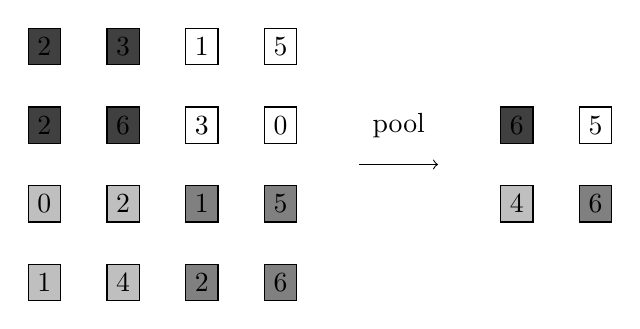
\begin{tikzpicture}
    \node[draw, fill=lightgray] (x00) at (0,0) {$1$};
    \node[draw, fill=lightgray] (x10) at (1,0) {$4$};
    \node[draw, fill=gray] (x20) at (2,0) {$2$};
    \node[draw, fill=gray] (x30) at (3,0) {$6$};
    \node[draw, fill=lightgray] (x01) at (0,1) {$0$};
    \node[draw, fill=lightgray] (x11) at (1,1) {$2$};
    \node[draw, fill=gray] (x21) at (2,1) {$1$};
    \node[draw, fill=gray] (x31) at (3,1) {$5$};
    \node[draw, fill=darkgray] (x02) at (0,2) {$2$};
    \node[draw, fill=darkgray] (x12) at (1,2) {$6$};
    \node[draw, fill=white] (x22) at (2,2) {$3$};
    \node[draw, fill=white] (x32) at (3,2) {$0$};
    \node[draw, fill=darkgray] (x03) at (0,3) {$2$};
    \node[draw, fill=darkgray] (x13) at (1,3) {$3$};
    \node[draw, fill=white] (x23) at (2,3) {$1$};
    \node[draw, fill=white] (x33) at (3,3) {$5$};

    \draw [->, text=pool] (4,1.5) to (5,1 .5);
    \node[draw=none] at (4.5,2) {pool};
    \node[draw, fill=darkgray] (x63) at (6,2) {$6$};
    \node[draw, fill=lightgray] (x62) at (6,1) {$4$};
    \node[draw, fill=white] (x73) at (7,2) {$5$};
    \node[draw, fill=gray] (x72) at (7,1) {$6$};
    \end{tikzpicture}
    \caption{Example of a max-pooling operation.}
    \label{fig:maxpool}
\end{figure}

\paragraph{Global pooling}
\label{p:global.pooling}
While a \gls{cnn} of stacked convolutional layers is a powerful hierarchical feature extractor, the output structure is not suited for the most tasks \glspl{cnn} are used for. Note that the output feature matrix at the end of the convolutional layers is 3-dimensional, while most tasks require flat vectors. A common task is image classification, which requires as output a vector consisting of as many entries as there are classes (as described in \Cref{subsubsec:classification}. There are two ways of restructuring the 3-dimensional feature matrix into such a vector. The first is \emph{global pooling} \citep{DBLP:journals/corr/LinCY13}, which is a pooling layer with a receptive field size that is equal to the total size of the feature matrix. This intuitively reduces the spatial dimensions of the output feature map (width and height, respectively) to 1. Since the receptive field size is very large, average-pooling is used instead of max-pooling. Just as with local pooling layers, global pooling does not change the non-spatial dimension of the vector. Hence, the channel dimension size of the global pooling output vector is equal to the filter size of the preceding convolutional layer $f_{n-1}$, which is a hyperparameter that can be freely chosen. In other words, the output of the global pooling layer is of dimensions $1\times1\times f_{n-1}$. Since the spatial dimensions are 1, this matrix can be squeezed into a vector of dimension $f_{n-1}$. Therefore, by setting the filter size of the ultimate convolutional layer $f_{n-1}$ to the output size required for the specific downstream task $l$ (for image classification, this would be the number of classes) and applying global pooling afterwards, the output of the \gls{cnn} can be structured in a way that is suitable for downstream tasks. Note, that this requires very little additional parameters. As the global pooling layer is parameter-free and parameters in a convolutional layer are shared across space, the parameters added to the network are equivalent to the parameters of the final convolutional layer $c^2*f_{n-2}*f_{n-1}$, where $f_{n-1}=l$.

A different way to restructure the 3-dimensional output matrix of convolutional layers $\textbf{o}\in\mathbb{R}^{W\times H\times f_{n-1}}$ is to directly flatten it into a vector $\textbf{o}\in\mathbb{R}^{W*H*f_{n-1}}$, which is a differentiable operation. This is then followed up by a fully connected hidden layer with a size equivalent to the required output size $l$. The output of this layer would then be $l$. While this is conceptionally simpler than the global pooling approach described above, it introduces more parameters. Since the layer is fully connected, this approach requires $W*H*f_{n-1}*l$ parameters, while the global pooling approach only requires $c^2*f_{n-2}*f_{n-1}$ parameters, where $c\ll W$ and $c\ll H$. Furthermore, since the spatial dimensions are reduced to 1 in a parameter-free way, the global pooling approach is more robust to spatial translations than the fully connected approach.

\paragraph{Strided convolution}
The convolutional layers described above use the convolution operation defined in \Cref{eq:conv}. This convolution is a special case of a strided convolution with a stride of $s=1$. Intuitively, the receptive field on which the kernel (or, filter) is applied on starts at the beginning of the width dimension and is moved horizontally by successive steps in the width dimension. After it reaches the end of the input matrix in the width dimension, it is moved vertically by one step in the height dimension and back to the beginning in the width dimension. Now, the process repeats until the receptive field has traversed the whole input map.

\begin{equation}
\label{eq:stridedconv}
    \textbf{o}_{i,j}=\sum_{k=0}^c\sum_{l=0}^c \textbf{w}_{k,l} \textbf{x}_{(s-1)*i+k,(s-1)*j+l}
\end{equation}

\begin{figure}
    \centering
    \includegraphics{graphics/no_padding_strides_00.pdf}
    \includegraphics{graphics/no_padding_strides_01.pdf}
    \caption{Example of strided convolution without padding by \citet{dumoulin2016guide}. The left image depicts the receptive field used to compute the output element at location (1,1) in the output map. The right image depicts the receptive field used to compute the output element at location (2,1).}
    \label{fig:stridedconv}
\end{figure}

The step size by which the receptive field is moved across the input map is also called \emph{stride}. In strided convolutions, the stride is a hyperparameter that can be freely changed. This operation is defined in \Cref{eq:stridedconv}. In \Cref{eq:stridedconv}, the stride is denoted by $s \in [1,\min(W,H)]$. Note that setting the stride to $s=1$ eliminates the stride term, leading to the convolution defined in \Cref{eq:conv}. Setting the stride $s>1$ leads to a larger spacing between the receptive fields, which effectively reduces the amount of times the kernel is applied in order to produce an entry in the output matrix. Therefore, this leads to an output matrix that is smaller than the input matrix. In other words, strided convolution with $s>1$ leads to a \emph{downsampling} of the input matrix. In this aspect, it is quite similar to a pooling operation. An example of strided convolution for $s=2$ is depicted in \Cref{fig:stridedconv}.

\paragraph{Transposed Convolution}
The transposed convolution (also called deconvolution or fractionally strided convolution) operation is the inverse to strided convolution. While strided convolution downsamples the input matrix and therefore reduces the spatial dimensions, transposed convolution upsamples the input matrix in order to increase the spatial dimensions. A visual example of transposed convolution can be seen in \Cref{fig:deconvolution}. Intuitively, the input matrix is padded with empty (or, zero-valued) elements in order to produce an output matrix with increased spatial dimensions. Here, the stride hyperparameter can be interpreted as the stride of the output matrix instead of the input matrix.

\begin{figure}
\centering
    \includegraphics[width=.3\textwidth]{graphics/no_padding_no_strides_transposed_00.pdf}
    \includegraphics[width=.3\textwidth]{graphics/no_padding_no_strides_transposed_01.pdf}
    \caption{Example of a transposed convolution without padding by \citet{dumoulin2016guide}. The left image depicts the receptive field used to compute the output element at location (1,1) in the output map. The right image depicts the receptive field used to compute the output element at location (2,1).}
    \label{fig:deconvolution}
\end{figure}


\paragraph{CoordConv}
\label{subsec:bg.cnn.coordconv}
\begin{figure}
    \centering
    \includegraphics[width=\textwidth]{graphics/coordconv.pdf}
    \caption{Comparison of a conventional convolution layer and a CoordConv layer for input data in 2-dimensional space \citep{DBLP:conf/nips/LiuLMSFSY18}.}
    \label{fig:coordconv}
\end{figure}
An important property of convolutional layers is that they are invariant to spatial translation. However, for some tasks, this property is actually harmful. A simple example of such a task is mapping carthesian coordinates into one-hot pixel encodings, i.e., to generate an image in which the pixel at the input location is marked. In order to relax translation-invariance, \citet{DBLP:conf/nips/LiuLMSFSY18} introduced the CoordConv layer, which is depicted in \Cref{fig:coordconv}. Let $\textbf{x}\in\mathbb{R}^{W\times H\times C}$ be the input matrix to a convolutional layer. In order to preserve spatial information, explicit coordinate data is concatenated to the non-spatial dimension of the input matrix. In the usual case of 2-dimensional space, the location in space can be represented by two coordinates $(i,j)$, where $i\in [0,W)$ denotes the location in the width dimension and $j\in [0,H)$ denotes the location in the height dimension. For each spatial axis, a matrix $\mathbf{c}\in R^{W\times H}$ is concatenated to the depth dimension of $x$. In the 2-dimensional case, one coordinate matrix $\mathbf{c}_i$ is successively filled with increasing integers column-wise, while another coordinate matrix $\mathbf{c}_j$ successively filled with increasing integers row-wise. Now, by linearly combining the concatenated coordinate vectors, it is possible to uniquely identify the spatial location of each element in the original input data. In practice, the values in the coordinate vectors $c\in\mathbf{c}$ are scaled to $c\in[-1,1]$ in order to fit the scale of other input data.

Since CoordConv layers - just like convolutional layers - are fully connected in the non-spatial dimension, the explicit concatenated spatial information is used in the computation of every element in the output matrix. Since the connection weights to the coordinate vectors are freely changeable, the model is able to learn whether to use spatial information depending on the task. \citet{DBLP:conf/nips/LiuLMSFSY18} showed that CoordConv layers outperform conventional convolutional layers on a variety of tasks such as image generation, object detection and image classification.

\paragraph{1-dimensional convolution}

Motivated by a desire to apply \glspl{cnn} on sequential data such as text and inspired by \glspl{tdnn} \citep{DBLP:conf/interspeech/BottouFBL89}, \citet{DBLP:journals/jmlr/CollobertWBKKK11} introduce 1-dimensional convolutional layers, which operate on only one spatial dimension. This makes it possible to apply convolutions on sequential (or, temporal) input data, which is often arranged using using 2-dimensional matrices $\mathbf{x}\in\mathbb{R}^{t\times f}$, where $t$ is the sequence length and $f$ is the number of features per element in the sequence. By interpreting $t$ as singular spatial dimension (i.e., assuming linear space along a single axis), it is possible to define 1-dimensional (or, temporal) convolutional layers that perform the same operations as 2-dimensional convolutional layers do on input data in 2-dimensional space.

\begin{equation}
\label{eq:conv1d}
    h_{i,j}=\sum_{k=0}^c \mathbf{w}_{j,k}\mathbf{x}_{i+k}
\end{equation}
\begin{figure}
    \centering
    \includegraphics[width=\textwidth]{graphics/conv1d.pdf}
    \caption{Schema of a 1-dimensional convolution.}
    \label{fig:conv1d}
\end{figure}


Let $\mathbf{x}\in\mathbb{R}^{t\times f}$ be the input sequence, $c$ denote the receptive field size and $\mathbf{h}\in\mathbb{R}^{t_h\times f_h}$ be the hidden layer output, where just like in 2-dimensional convolutional layers $t_h=t$ assuming padding is used and $f_h$ is the filter size. Then, the 1-dimensional convolutional layer is defined by \Cref{eq:conv1d}, where $h_{i,j}$ is the element at location $(i,j)$ in the output matrix $\mathbf{h}$ and $\mathbf{w}\in\mathbb{R}^{f_h\times c\times f}$ is the kernel, i.e., the parameters or connection weights. The output $\mathbf{h}$ has the same dimensionality as the input sequence, with a singular spatial (or, temporal) dimension and a channel dimension the size of the numbers of filters. This way, the output of this 1-dimensional convolutional layer can in turn be used as input for a successive 1-dimensional convolutional layer, just like 2-dimensional convolutional layers. A visual example can be seen in \Cref{fig:conv1d}.

\subsubsection{Architectures}
\label{subsec:bg.cnn.arch}

While the above sections introduced the main building blocks of \glspl{cnn}, this section describes \gls{cnn} architectures that combine them in a way that has led to empirical successes \citep{ILSVRC15}.

As described in \Cref{subsec:bg.nn}, \glspl{mlp} generally perform better the deeper they are, i.e., the more hidden layers are used. This is especially true for \glspl{cnn}, which are explicitly designed to exhibit hierarchical representation learning \citep{DBLP:journals/pr/FukushimaM82,DBLP:conf/cvpr/SzegedyLJSRAEVR15}. However, it has been shown that \glspl{cnn} that exceed a certain depth threshold actually underperform \citep{DBLP:conf/cvpr/HeZRS16}. In order to solve this problem, \citet{DBLP:conf/cvpr/HeZRS16,DBLP:conf/nips/SrivastavaGS15} propose to computationally connect layer outputs that are far away in the graph. This way, the learning signal does not just propagate between directly neighbouring layers, but can \emph{skip} layers. Hence, this connection of layers at different depths is called \emph{skip connection}. Skip connections increase the diversity of paths to deeper layers, resulting in improved accuracy and faster convergence during training.

\begin{figure}
    \centering
    \includegraphics{graphics/residual_block.pdf}
    \caption{Residual learning block \citep{DBLP:conf/cvpr/HeZRS16}.}
    \label{fig:residual_block}
\end{figure}

A simple skip connection proposed by \citet{DBLP:conf/cvpr/HeZRS16} is the residual connection, i.e., to simply sum the outputs of a hidden layer with the outputs of a hidden layer at a different depth. This residual connection is depicted in \Cref{fig:residual_block}. This figure shows two arbitrary hidden layers in a deep \gls{cnn}, with $\mathbf{x}$ denoting the output of the preceding hidden layer, which is used as input for the first hidden layer. At the end of the block, the output of the second hidden layer is connected through addition with the identity of the output of the hidden layer preceding this block. This addition with the identity function is parameter-free and differentiable. This way, there are now two paths the signal can be propagated to, without increasing the parameter size. One path includes the intermediate first hidden layer, while the other one skips it. Note, that for the matrix addition to work both summands need to have the same dimension.

The ResNet architecture proposed by \citep{DBLP:conf/cvpr/HeZRS16} stacks a large number of residual blocks in order to form a deep \gls{cnn} which does not suffer from convergence issues. This \gls{cnn} architecture is depicted in \Cref{fig:resnet34}. The \gls{cnn} consists of an initial convolutional layer, followed by a max-pooling layer, 16 residual blocks, a gloval average-pooling layer and an ultimate fully connected layer. In total, this architecture consists of 34 layers. The input image is resized to a width and height of 224 pixels. This is a common practice for \glspl{cnn}, since high resolution input images would lead to a higher number of parameters. The first convolutional layer performs strided convolution with a stride of $s=2$, receptive field size of $c=7$ and a channel size (or, filter size) of $f=64$. Since $s=2$, the output feature map of this layer has a width and height of $224/2=112$. Afterwards, the max-pooling layer with a receptive field size of 2 further reduces this to $112/56$. This output is then used as input for the first of a sequence of 16 residual blocks. The convolutional layers in all residual blocks are performed with a receptive field size of $c=3$. Intermittently, a strided convolution with $s=2$ is used in order to halve the output size. The convolutional layer immediately following such a halving has double the filter size of the preceding layer $f_{i+1}=f_i*2$. All other convolutional layers have the same filter size as their predecessor.

\begin{figure}
\centering
    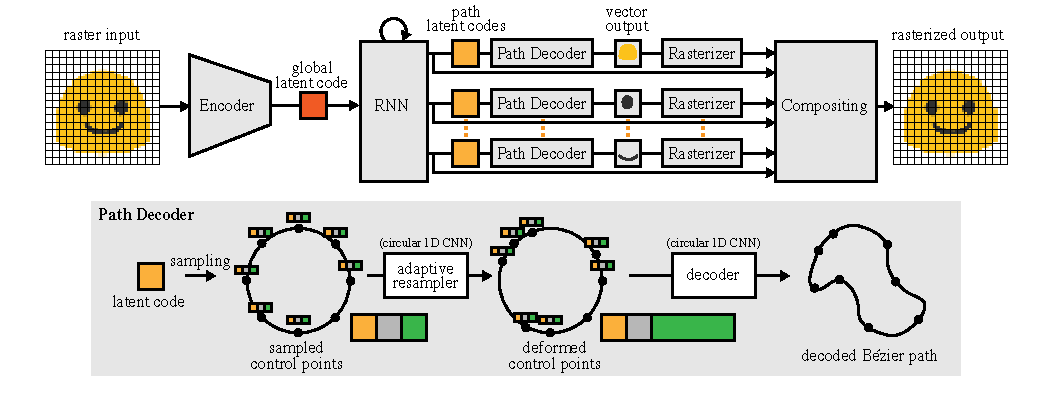
\includegraphics{graphics/arch.pdf}
    \caption{ResNet architecture design with 34 layers and residual blocks instead of bottleneck blocks \citep{DBLP:conf/cvpr/HeZRS16}.}
    \label{fig:resnet34}
\end{figure}

%\begin{wrapfigure}{l}{.4\textwidth}
%    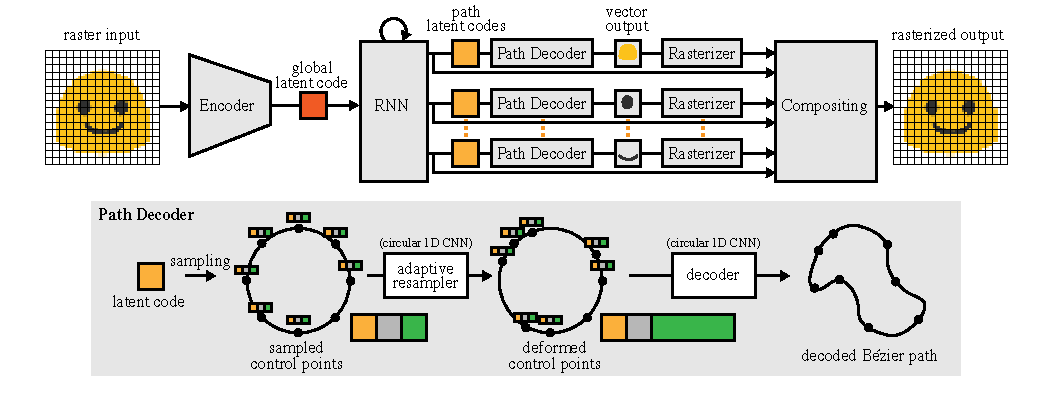
\includegraphics{graphics/arch.pdf}
%    \caption{ResNet architecture design with 34 layers and residual blocks instead of bottleneck blocks \citep{DBLP:conf/cvpr5/HeZRS16}.}
%    \label{fig:resnet34}
%\end{wrapfigure}

Recall that for addition in the residual connection, the summands need to have the same dimension. This means, given that layers $i$ and its successor $j$ have a different filter size than preceding layer $h$, a residual connection of $h$ to $j$ is not possible. In order to enable such a connection, a convolutional layer with receptive field size $c=1$ is applied on the output of the preceding layer $\textbf{o}_h$ before being added to the output of the connected layer $\textbf{o}_j$. Crucially, the filter size of this 1x1-convolution is identical to the the filter size of the succeeding layers $i$ and $j$. Since $c=1$, the convolution preserves the spatial dimensions of the output, but changes the filter size to match layers $i$ and $j$. This \emph{projection shortcut} enables residual connections across layers with different filter sizes, but also introduces (a low amount of) additional parameters. It is preferable to keep filter sizes constant in order to use parameter-free residual connections as much as possible. In the few instances in which the filter size changes in the ResNet architecture, projection shortcuts have to be used immediately afterwards. These are indicated by dotted arrows in \Cref{fig:resnet34}.

%Note that the output feature map at the end of the convolutional layers is 3-dimensional. This output structure is not suited for the most tasks \gls{cnn} are used for, which require 1-dimensional vectors. Taking the example of image classification, which requires as output a one-dimensional vector consisting of as many entries as there are classes.

Since the ResNet architecture was trained and tested for an image classification task, the output feature map has to be structured into a vector with a cardinality of 1000 (which is the number of classes in the ImageNet dataset \citep{ILSVRC15}). In order to achieve this, global average-pooling is used in order to reduce the output feature matrix into a vector with cardinality 512, which is the filter size of the ultimate convolutional layer. Afterwards, a fully connected layer is used to produce an output vector of cardinality 1000.

\begin{figure}
    \centering
    \includegraphics{graphics/block_deeper.pdf}
    \caption{Comparison of a residual block (left) and a bottleneck block (right) \citep{DBLP:conf/cvpr/HeZRS16}.}
    \label{fig:bottleneck}
\end{figure}

The 34-layer ResNet described above was empirically shown to solve the degradation problems experienced by deep \gls{cnn} without residual connections \citep{DBLP:conf/cvpr/HeZRS16}. Therefore, \citet{DBLP:conf/cvpr/HeZRS16} introduced ResNet architectures that were even deeper. For computational efficiency, residual blocks are replaced by \emph{bottleneck} blocks, which are depicted in \Cref{fig:bottleneck}. Here, the two convolutional layers of residual blocks are replaced with three convolutional layers. The first convolutional layer has a receptive field size $c=1$ and a filter size $f=64$. This layer solely serves to reduce the filter size. The succeeding convolutional layer with a receptive field size of 3 performs the usual feature extraction on this reduced filter size. The final convolutional layer again has a receptive field size of 1 and a filter size of 256. As an inverse to the first layer, it serves to increase the filter size to the same size it is in output of the preceding block. This way, the convolutional layer performing feature extraction is a bottleneck with smaller input and output filter size. This serves both as regularization and to increase computational efficiency.

By replacing all residual blocks in the ResNet-34 architecture with bottleneck blocks, the number of layers is increased to 50. \citet{DBLP:conf/cvpr/HeZRS16} show that this model already performs better than ResNet-34. \citet{DBLP:conf/cvpr/HeZRS16} build even deeper models by stacking more bottleneck blocks, arriving at a ResNet model with 152 layers, which yielded the best empirical results.

The ResNet architecture has been widely used to create deep \gls{cnn} architectures. There exists a range of extensions and modifications to the original architecture, including ResNetv2 \citep{DBLP:conf/eccv/HeZRS16}, Wide ResNet \citep{DBLP:conf/bmvc/ZagoruykoK16}, ResNeXt \citep{DBLP:conf/cvpr/XieGDTH17} and most recently ConvNeXt \citep{DBLP:conf/cvpr/0003MWFDX22}.


\subsection{Recurrent Neural Networks}
\label{subsec:bg.rnn}

While the \gls{mlp} is a general purpose architecture and the \gls{cnn} has an inductive bias for spatial data, the recurrent neural network is a neural network architecture with an inductive bias for sequential (or, temporal) data. The original architecture introduced by \citet{Rumelhart1986} equips neural networks with memory capabilities. In contrast to other neural network architectures such as \glspl{mlp} or \glspl{cnn}, individual forward passes on inputs are not independent. Let $\mathbf{x}_n$ be an input sequence. Just like with neural networks, recurrent neural networks perform a forward pass according to $f(\mathbf{x}_0; \boldsymbol{\theta})$. Contrary to neural networks, the forward pass for the next input $\mathbf{x}_1$ depends on the forward pass of the previous input, i.e., $f(\mathbf{x}_1;\boldsymbol{\theta};f(\mathbf{x}_0; \boldsymbol{\theta}))$. This loop-like functionality enables \glspl{rnn} to take previous inputs and predictions into account when computing new predictions. The simple \gls{rnn} architecture is defined in \Cref{eq:vanillarnn.h,eq:vanillarnn.o}.

\begin{equation}
\label{eq:vanillarnn.h}
        \mathbf{h_t} = \phi(\mathbf{h}_{t-1} \boldsymbol{\theta}_h + \mathbf{x}_t \boldsymbol{\theta}_x)
\end{equation}

\begin{equation}
\label{eq:vanillarnn.o}
        \mathbf{o}_t = \mathbf{h_t} \boldsymbol{\theta}_o
\end{equation}

Note that all variables in \Cref{eq:vanillarnn.h,eq:vanillarnn.o} are temporal, i.e., depend on $t$. Only the learnable parameters $\boldsymbol{\theta}$ are constant. $\mathbf{h}_t$ is the state of recurrent neural network. It represents all individual inputs and state changes up to  $\mathbf{x}_t$. The output $\mathbf{o}_t$ is computed by taking the current state $\mathbf{h}_t$ into account. Thus, a \gls{rnn} can natively handle temporal inputs.

Recurrent neural networks are optimized in the same way as standard neural networks. However, due to the temporal component introduced in \Cref{eq:vanillarnn.h,eq:vanillarnn.o}, the gradient can not be computed using standard backpropagation. The gradients needed for loss function optimization are computed using the backpropagation-through-time algorithm \citep{robinson:utility}.

In practice, standard recurrent neural networks are not able to generalize well and do not take long-term dependencies into account because they suffer from vanishing or exploding gradients \citep{hochreiterdipl,Bengio:1994:LLD:2325857.2328340}.

\subsubsection{Gated Recurrent Units}

In order to alleviate the convergence problems of standard recurrent neural networks, \citet{Hochreiter:1997:LSM:1246443.1246450} introduced the \gls{lstm} recurrent neural network. In addition to the hidden state $\mathbf{h}_t$, it introduces a cell state $\mathbf{c}$ and a corresponding set of update equations which do not suffer from gradient problems. A simplified variant of the \gls{lstm} architecture are \glspl{gru} \citep{cho14}. Its authors claim that \glspl{gru} work better than \glspl{lstm}. \Crefrange{eq:gru1}{eq:gru4} detail the update procedure similar to \Cref{eq:vanillarnn.h,eq:vanillarnn.o}. Note that $\mathbf{o}_t = \mathbf{h}_t$.

\begin{equation}
\label{eq:gru1}
        \mathbf{z}_t = \phi_\text{sigmoid}([\mathbf{h}_{t-1},\mathbf{x}]\boldsymbol{\theta}_z)
\end{equation}

\begin{equation}
\mathbf{r}_t = \phi_\text{sigmoid}([\mathbf{h}_{t-1},\mathbf{x}]\boldsymbol{\theta}_r)
\end{equation}

\begin{equation}
\mathbf{\tilde{h}}_t = \phi_\text{tanh}([\mathbf{r}_t \mathbf{h}_{t-1},\mathbf{x}]\boldsymbol{\theta}_h)
\end{equation}

\begin{equation}
\label{eq:gru4}
\mathbf{h}_t = (1 - \mathbf{z}_t) \mathbf{h}_{t-1} + \mathbf{z}_t \mathbf{\tilde{h}}_t
\end{equation}

It is still unknown whether \glspl{gru} truly improve upon \glspl{lstm}. A large-scale study \citep{7508408} compared \gls{lstm} variants on speech recognition, handwriting recognition and music modeling tasks and found no significant difference. Another study \citep{pmlr-v37-jozefowicz15} used a different hyperparameter optimization algorithm and compared \glspl{lstm} and \glspl{gru} on arithmetic, XML modeling, language modeling and music modeling tasks. They conclude that \glspl{gru} perform better than \glspl{lstm}.

\subsubsection{CNN or RNN?}

As discussed in \Cref{subsec:bg.cnn} and \Cref{subsec:bg.rnn}, both 1-d convolutional and recurrent neural networks can handle temporal data. While only \glspl{rnn} can properly handle sequences of unknown length, for input data of fixed length, it is of interest to know which architecture is better suited. This comparison was investigated by \citet{2017arXiv170201923Y,2018arXiv180301271B}. Both come to the conclusion that 1-dimensional \glspl{cnn} lead to better and faster convergence than \glspl{rnn} on sequence classification tasks. Keep in mind, however, that the empirical results using toy problems might not generalize.


\subsection{Transformer}
\label{subsec:bg.tf}

The Transformer introduced by \citet{DBLP:conf/nips/VaswaniSPUJGKP17} is a neural network architecture that essentially combines the advantages of \glspl{rnn} and \glspl{cnn}. Like \glspl{rnn}, it can be used for sequential data, but like \glspl{cnn} it can be efficiently computed on \glspl{gpu} using matrix multiplications. The Transformer consists almost solely of \emph{self-attention} modules, which are explained below.

\subsubsection{Self-Attention}
Attention is a general purpose mechanism for neural networks introduced by \citet{DBLP:journals/corr/BahdanauCB14} and was originally intended for machine translation \glspl{rnn}. It allows to assign each element $\mathbf{x}_i$ of an input set $\mathbf{X}$ an attention weight $\alpha_i$. Crucially, this mechanism is differentiable, so it can be fitted along with the neural network model.

Originally, attention was intended to compute values using both an input sequence (text in \citet{DBLP:journals/corr/BahdanauCB14}) and an output sequence (\gls{rnn} hidden states in \citet{DBLP:journals/corr/BahdanauCB14}). However, the form of attention used for Transformers operates over a single input sequence only. This form is called \emph{self-attention} (or inter-attention).

Let $\mathbf{X} \in \mathbb{R}^{n\times m}$ be a set of $n$ elements with $m$ features. In the general form, the self-attention mechanism transforms $\mathbf{X}$ into a \emph{contextualized} set $\mathbf{Y} \in \mathbb{R}^{n \times m}$. The resulting set is of the same length as $\mathbf{X}$ and $\mathbf{y}_i \in \mathbf{Y}$ can be interpreted as representing the value of $\mathbf{x}_i \in \mathbf{X}$ taking into consideration all other elements of $\mathbf{X}$. Mathematically, this can be achieved by first computing \emph{attention weights} $\mathbf{A}$ as the dot-product of $\mathbf{X}$ with itself, as can be seen in \Cref{eq:attn}. This equation uses the unit softmax function defined in \Cref{eq:softmax} to produce a pseudo-probability distribution from the unbounded attention scores, i.e., to bound them to $[0,1]$ and let them sum to 1. The contextualized set $\mathbf{Y}$ can then be computed as the weighted sum of $\mathbf{X}$ using the attention weights, as defined in \Cref{eq:attn.res}.

\begin{equation}
        \label{eq:attn}
        \mathbf{A} = \text{softmax}(\mathbf{X}\mathbf{X}')
\end{equation}

\begin{equation}
        \label{eq:softmax}
        \text{softmax}(\mathbf{x})_i=\frac {\exp(x_i)}{\sum_{j=1} ^{|\mathbf{x}|} \exp(x_j)}
\end{equation}

\begin{equation}
        \label{eq:attn.res}
        \mathbf{y}_i = \sum_{j=1}^{n} \alpha_{ij} \mathbf{x}_j
\end{equation}

In conclusion, the element $\mathbf{y}_i \in \mathbf{Y}$ is computed by \emph{attending} to individual elements of $\mathbf{X}$ with different weights. This attention variant using a weighted sum introduced here is also called \emph{soft attention}, since all input elements contribute to the output. There also exists hard attention described in \citet{pmlr-v37-xuc15}, which explicitly selects elements instead of using a weighted sum of all elements. Since this is not differentiable, it is more complex to integrate it in the optimization procedure.

This self-attention mechanism can be further extended with learnable parameters. Notice in \Cref{eq:attn,eq:attn.res} that $\mathbf{X}$ is used three times in the self-attention mechanism. Different learnable parameters $\mathbf{W}\in\mathbb{R}^{m\times m}$ are used for these three occurrences.  To distinguish them more easily, these are defined analogous to a continuous dictionary as query $\mathbf{Q}=\mathbf{X}\mathbf{W_Q}$, key $\mathbf{K}=\mathbf{X}\mathbf{W_K}$ and value $\mathbf{V}=\mathbf{X}\mathbf{W_V}$. In \Cref{eq:attn.kqv}, the query and the key are matched to produce a compatibility (i.e., the attention weights), which is then used in \Cref{eq:attn.res.kqv} to retrieve the values. It is also clear that this attention variant is called \emph{self-attention} because $\mathbf{Q}$, $\mathbf{K}$ and $\mathbf{V}$ are computed using the same input $\mathbf{X}$.

\begin{equation}
        \label{eq:attn.kqv}
        \mathbf{A} = \text{softmax}(\mathbf{Q}\mathbf{K}')
\end{equation}

\begin{equation}
        \label{eq:attn.res.kqv}
        \mathbf{Y} = \mathbf{A} \mathbf{V}
\end{equation}

The self-attention variant described until now is called \emph{dot-product attention} \citep{DBLP:conf/emnlp/LuongPM15,DBLP:journals/corr/GravesWD14}. There also exists \emph{additive attention} \citep{DBLP:journals/corr/BahdanauCB14}. This approach first computes attention scores $s_{ij}$ by concatenating $\mathbf{q_i}$ and $\mathbf{k'_j}$ and using the concatenated vector as an input to a single layer \gls{mlp}. This can be seen in \autoref{eq:attn.add}. In this equation, $\mathbf{q}_i \| \mathbf{k}_j\in \mathbb{R}^{nm}$, $\mathbf{W_A}\in \mathbb{R}^{nm}$ are the learnable parameters and $\phi$ is a non-linearity such as the tanh function. Then in \Cref{eq:attn.add.soft} the softmax function is used to compute the attention weights.

\begin{equation}
        \label{eq:attn.add}
        s_{ij} = \phi(\mathbf{W_A}[\mathbf{q}_i \| \mathbf{k}_j])
\end{equation}

\begin{equation}
        \label{eq:attn.add.soft}
        \alpha_{ij}=\text{softmax}(\mathbf{s})_{ij}
\end{equation}

In practice, additive attention leads to better results than dot-product attention if the feature dimension $m$ is large \citep{britz-etal-2017-massive}. However, it can be seen that, to compute the entire attention matrix $\mathbf{A}$, additive
attention needs to use the neural network $nm$ times. This cannot be restructured into a single matrix multiplication due to the non-linearity. Contrary to that, dot-product attention can simply be computed using a matrix multiplication, which is more suited for GPU workloads. To remedy this situation, \emph{scaled} dot-product attention \citep{DBLP:conf/nips/VaswaniSPUJGKP17} has been introduced. This simply normalizes the dot product by $1/\sqrt{m}$ to counteract the adverse effect of large values of $m$ and has largely replaced additive attention.

\begin{equation}
        \label{eq:attn.scal.kqv}
        \mathbf{A} = \text{softmax}\left(\frac{\mathbf{Q}\mathbf{K}'}{\sqrt{m}}\right)
\end{equation}

Another way of stabilizing self-attention is multi-head attention \citep{DBLP:conf/nips/VaswaniSPUJGKP17}, which is analogous to using multiple channels in \glspl{cnn}. Multiple heads of the self-attention function $h$ are computed in parallel using different learnable parameters in \autoref{eq:attn.multi}. The $h$ output matrices are concatenated and projected to the original dimension $\mathbb{R}^{n\times m}$ using the learnable linear transformation $\mathbf{W}_\mathbf{Y}\in\mathbb{R}^{n \times nh}$ in \autoref{eq:attn.multi.res}. Intuitively, this allows to attend to different embeddings simultaneously. \citet{DBLP:conf/nips/VaswaniSPUJGKP17} set $h=8$ for their architecture.

\begin{equation}
        \label{eq:attn.multi}
        \mathbf{Y}^{\text{head}_i}=\text{Self-Attention}(\mathbf{X}; \mathbf{W}^i_\mathbf{Q}, \mathbf{W}^i_\mathbf{K}, \mathbf{W}^i_\mathbf{V}).
\end{equation}

\begin{equation}
        \label{eq:attn.multi.res}
        \mathbf{Y}= \mathbf{W}_\mathbf{Y}  \left(\|_{i=0}^{h} \mathbf{Y}^{\text{head}_i}\right) 
\end{equation}


The main computational problem of standard self-attention is that its space and time complexity is quadratic in the set length $n$. This quickly becomes a problem for larger values of $n$. Multiple approaches were proposed to modify self-attention to achieve lower runtime, memory or IO complexity \citep{DBLP:conf/iclr/ChoromanskiLDSG21,DBLP:conf/nips/DaoFERR22}.

Another approach to solve this computational problem is local attention \citep{DBLP:conf/emnlp/LuongPM15}. The self-attention variant described above can be seen as \emph{global} attention, since it uses the entire input set $\mathbf{X}$ to compute each output vector $\mathbf{y}_i$. In local attention, only a constant number of neighbours is used. This is computationally more efficient, but restricts the contextualized output vectors from taking longer-range dependencies into account. In practice, most works utilize standard self-attention and deal with the complexity by increasing hardware resources.

\subsubsection{Standard Transformer}

\begin{figure}[h]
        \centering
        \includegraphics[width=.3\textwidth]{graphics/ModalNet-21}
        \caption{Transformer architecture by \citet{DBLP:conf/nips/VaswaniSPUJGKP17}.}
        \label{fig:transformer}
\end{figure}

While (self-)attention was originally only used as an add-on for \glspl{rnn}, the Transformer architecture introduced by \citet{DBLP:conf/nips/VaswaniSPUJGKP17} consists solely of global scaled self-attention modules stacked with an \gls{mlp}. They showed that this is not only simpler but actually preferable to using \glspl{rnn}. While the Transformer uses a fixed number of self-attention modules, an \gls{rnn} requires $n$ sequential operations. This is an advantage, since it has been established that a shorter path length between two positions makes it easier to learn long-range dependencies \citep{5264952}.

The Transformer architecture is depicted in \Cref{fig:transformer} and consists of stacked transformer blocks, with each block consisting of multi-head self-attention and layer normalization \citep{DBLP:journals/corr/BaKH16} (similar to batch normalization as described in \Cref{subsec:bg.nn.batchnorm}) followed by a simple \gls{mlp} and layer normalization. The \gls{mlp} is position-wise, i.e., it is applied to each output vector $\mathbf{y}_i$ individually. The architecture employs residual connections \citep{7780459} around each individual block step.

The Transformer architecture can be used for any kind of real-valued set data. Originally, it was intended for \gls{nlp} tasks and thus to beused with text data as input. However, text data is sequential in nature, while the Transformer architecture does not preserve order information due to the permutation-equivariant self-attention layers. This is similar to using 1-dimensional CoordConv layers as described in \Cref{subsec:bg.cnn.coordconv}. In order to be able to use sequential data, the Transformer architecture concatenates a positional encoding to each input element before applying self attention. The Transformer architecture employs global attention and thus computes the attention of all input pairs.

Since the Transformer continually leads to new successes in \gls{nlp} \citep{DBLP:conf/naacl/DevlinCLT19,DBLP:conf/nips/BrownMRSKDNSSAA20,DBLP:journals/corr/abs-2302-13971}, there have been numerous attempts to apply it on visual data. These \glspl{vit} perform comparably and in some cases outperform \glspl{cnn} on a variety of tasks such as image classification and object detection \citep{DBLP:conf/iclr/DosovitskiyB0WZ21,liu2021Swin}.


\subsection{Encoder-Decoder Framework}
\label{subsec:bg.vae}

An important general framework for generative deep learning architectures is the encoder-decoder framework. To motivate this, first, the \emph{autoencoder} architecture \citep{https://doi.org/10.1002/aic.690370209} is introduced.

Recall that neural networks are universal function approximators, i.e., they approximate an arbitrary real-valued ground truth function $F(\textbf{x})=\textbf{y}, F: \mathcal{X} \rightarrow \mathcal{Y}$ using freely changeable parameters $\boldsymbol{\theta}$ as $f(\mathbf{x};\boldsymbol{\theta})$. In many tasks, the input and output data are part of different vector spaces, e.g. in image classification $\mathbf{x}\in\mathcal{X}$ being an image and $\mathbf{y}\in\mathcal{Y}$ being the class probabilities. The autoencoder architecture was introduced by \citet{https://doi.org/10.1002/aic.690370209} to solve the task of condensing the input $\mathbf{x}$ into a an efficient (i.e., smaller) code $\mathbf{z}\in\mathcal{Z}$, which can be used to fully reconstruct $\mathbf{x}$. It must hold, then, that this code contains all essential information about the input data. This code is referred to as \emph{latent code}, or, since it is represented as a vector, \emph{latent vector}.

\begin{figure}
    \centering
    \includegraphics[width=\textwidth]{graphics/autoencoder.pdf}
    \caption{Schema of the autoencoder architecture.}
    \label{fig:autoencoder}
\end{figure}

For the purpose of finding efficient encodings, the autoencoder consists of two neural networks. The \emph{encoder} $e$ defined in \Cref{eq:autoencoder.enc} is an \gls{mlp} which maps the input $\mathbf{x}\in\mathcal{X}$ to the latent vector $\mathbf{z}\in\mathcal{Z}$ using freely changeable parameters $\boldsymbol{\theta}_e$. In turn, the \emph{decoder} $d$ defined in \Cref{eq:autoencoder.dec} is an \gls{mlp} which maps the latent vector $\mathbf{z}$ to an output vector $\mathbf{x'}\in\mathcal{X}$ with $\mathbf{x'}\approx\mathbf{x}$ (or, in the optimal case $\mathbf{x'}=\mathbf{x}$) using freely changeable parameters $\boldsymbol{\theta}_d$. The complete autoencoder is then defined by \Cref{eq:autoencoder} and depicted in \Cref{fig:autoencoder}. The autoencoder is optimized using gradient descent of a loss function measuring the distance between $\mathbf{x}'$ and $\mathbf{x}$ such as the $L^1$ or $L^2$ distance described in \Cref{subsec:bg.losses}. Furthermore, an important design consideration is that the latent vector is smaller than the input vector, since if $\dim(\mathbf{z})=\dim(\mathbf{x})$, the autoencoder might converge to the identity function as local optimum.


\begin{equation}
\label{eq:autoencoder.enc}
    \mathbf{z}=e(\mathbf{x};\boldsymbol{\theta}_e)
\end{equation}\begin{equation}
\label{eq:autoencoder.dec}
    \mathbf{x'}=d(\mathbf{z};\boldsymbol{\theta}_d)
\end{equation}
\begin{equation}
\label{eq:autoencoder}
    \mathbf{x'}=d(\mathbf{z};\boldsymbol{\theta}_d)=d(e(\mathbf{x};\boldsymbol{\theta}_e);\boldsymbol{\theta}_d)
\end{equation}

Autoencoders were proposed for dimensionality reduction, since the latent vector theoretically contains all necessary information of the input data in smaller form. This can be useful as a compression technique. Additionally, it is possible to apply vector space operations on the latent vector that might not have been possible or practical on the input data, such as linear transformations or distance measures. Furthermore, it is possible to use autoencoders for generative tasks by using the decoder of an optimized autoencoder on its own. By sampling an arbitrary $\mathbf{z}_k\in\mathcal{Z}$ and inputting it into an optimized $d$, it is possible to generate new output data $\mathbf{x}'_k\in\mathcal{X}$ that follows the same distribution of the training input data (e.g. if $\mathcal{X}$ is an image space, generating new images that are similar to the images in the training dataset). In turn, since the encoder is differentiable, optimized encoders can also be used on their own for downstream tasks. For this reason, autoencoders have found a wide range of applications \citep{DBLP:conf/ssst/ChoMBB14,DBLP:conf/iclr/TheisSCH17,doi:10.1126/science.1127647}.

By generalizing the autoencoder to inputs and outputs of different distributions, one arrives at the encoder-decoder framework \citep{DBLP:conf/nips/SutskeverVL14,FITPT283} as depicted in \Cref{fig:encoderdecoder}, which is used by a wide variety of recently successful neural network architectures such as the Transformer (as explained in \Cref{subsec:bg.tf}). As an example, \citet{DBLP:journals/corr/abs-1301-3781} use an encoder-decoder architecture to encode words (i.e., character sequences) into semantically meaningful latent vectors. The encoder-decoder framework is defined in \Cref{eq:encdec}, which is a generalization of \Cref{eq:autoencoder}. Note that the output vector $\mathbf{y}\in\mathcal{Y}$ of the decoder $d$ follows a different distribution than the input vector $\mathbf{x}\in\mathcal{X}$. Furthermore, the optimization objective is not $\mathbf{y}=\mathbf{x}$, as is the case in autoencoders, but is replaced with a task-dependent objective.

\begin{figure}
    \centering
    \includegraphics[width=\textwidth]{graphics/encoderdecoder.pdf}
    \caption{Schema of an architecture following the encoder-decoder framework.}
    \label{fig:encoderdecoder}
\end{figure}

\begin{equation}
\label{eq:encdec}
    \mathbf{y}=d(\mathbf{z};\boldsymbol{\theta}_d)=d(e(\mathbf{x};\boldsymbol{\theta}_e);\boldsymbol{\theta}_e)
\end{equation}


As an aside, there exist different versions of and modifications to the autoencoder architecture. Chief among them is the \gls{vae}, which attempts to normalize the latent space $\mathcal{Z}$ s.t. $\forall z_i\in\mathbf{z}\in\mathcal{Z}$, $z_i \sim \mathcal{N}(0,1)$, where $N(\mu,\sigma)$ is a normal distribution with mean $\mu$ and standard deviation $\sigma$. In order to achieve this, a loss term which calculates the  divergence between $\mathbf{z}$ and the standard-normal distribution $\mathcal{N}(0,1)$ is added to the autoencoder loss. Usually, \gls{kl} divergence \citep{10.1214/aoms/1177729694} is chosen as loss function.

\subsubsection{Feature Combination}
There exist encoder-decoder architectures with multiple encoders but only one decoder, most commonly if input from different modalities is used to generate a single output. In this case, multiple latent vectors have to be combined into a single latent vector suitable for consumption by the decoder. This is referred to as \emph{feature combination}, or \emph{feature fusion}. Two common types of feature combination are introduced in this section.

\begin{equation}
    \label{eq:concatfeaturefusion}
    \mathbf{z_o}= \mathbf{z}_0 | \mathbf{z}_1 | \dots | \mathbf{z}_N= |_{i=0}^N \mathbf{z}_i
\end{equation}

A simple feature combination technique is to concatenate the latent vectors into a single, latent vector, as defined in \Cref{eq:concatfeaturefusion}. This is parameter-free and quick to compute. Let $|\mathbf{z}_i|$ be the length of an input latent vector. Then the length of the output latent vector is $|\mathbf{z}_o| =\sum_i^N |\mathbf{z}_i|$. Hence, the combined latent vector is of a different length than the input vectors and quickly grows very long. If the decoder requires the latent vector to be of a specific length, or if the concatenated latent vector would be too long, \emph{learned} feature combination is preferable. In this technique, the concatenated latent vectors are input followed by a fully connected layer, which produces a combined latent vector of the hidden layer size, which can be set as a hyperparameter. It is defined by \Cref{eq:learnedfeaturefusion}, where $f$ is a fully connected hidden layer. Note, however, that depending on the length this introduces a considerable amount of parameters. As an aside, learned feature combination by concatenation is similar to additive attention as introduced in \Cref{eq:attn.add}.

\begin{equation}
    \label{eq:learnedfeaturefusion}
    \mathbf{z_o}=f(|_{i=0}^N \mathbf{z}_i;\boldsymbol{\theta})
\end{equation}

Note that there exists a wide range of feature combination types other than the ones explained above. As an example, the skip connections introduced in \Cref{subsec:bg.cnn.arch} are a kind of feature combination by addition.

